\documentclass[12p]{article}
\usepackage{a4wide} %strona formatu a4, szeroko wypełniona tekstem
\usepackage{amsmath} %dodatkowe komendy, np. \underset
\usepackage{polski} %polskie litery
\usepackage{graphicx} 
\usepackage{amssymb}
\usepackage{tikz}
\usepackage{adjustbox}
\usepackage{float}
\usepackage{lmodern}
\usepackage{amsmath}
\usepackage{pgfplots}
\usepackage{array}
\usepackage{makecell}
\usepackage{pgfplots}
\usepackage{seqsplit}
\usetikzlibrary{fit}
\usepackage{lipsum}
\thispagestyle{empty}
\usetikzlibrary{arrows}
\usepackage{tikz}
\usetikzlibrary{shapes.geometric, arrows}
\linespread{1.3}
\usepackage{geometry} 
\newgeometry{tmargin=3.5cm, bmargin=3.5cm, lmargin=4.5cm, rmargin=2.5cm}
\tikzstyle{prostokat} = [rectangle, rounded corners, minimum width=3cm, minimum height=1cm,text centered, draw=black]
\tikzstyle{arrow} = [thick,->,>=stealth]

\begin{document}

\thispagestyle{empty}
\vspace*{\fill}
\begin{flushright}
Składam serdeczne podziękowania\\
Panu prof. Rafałowi Długoszowi\\
za cenne porady, poświęcony czas,\\
cierpliwość oraz pomoc w trakcie\\
powstawania pracy dyplomowej.
\end{flushright}
%Składam serdeczne podziękowania
%Pani dr Małgorzacie Obarowskiej
%za cenne porady, poświęcony czas,
%cierpliwość oraz pomoc w trakcie
%powstawania pracy dyplomowej.
\newpage
\tableofcontents
\newpage


\section{Cel i zakres pracy}
\quad Celem pracy jest przedstawienie algorytmów kryptograficznych, budowy systemów wbudowanych oraz implementacja algorytmu DES na systemie wbudowanym wraz ze zmierzeniem jego wydajności w zależności od rozmiaru szyfrowanych danych. Praca składa się z części teoretycznej, będącej wprowadzeniem do zagadnień kryptograficznych oraz budowy systemów wbudowanych i części praktycznej, w której przedstawiono charakterystykę wybranego systemu wbudowanego oraz implementację algorytmu DES wraz z przedstawieniem jego wydajności. Praca została podzielona na na dwie części: część teoretyczną, która składa się z dwóch rozdziałów i część praktyczną, która zawiera również dwa rozdziały. 

W pierwszej części teoretycznej w rozdziale 2 opisano najczęstsze ataki na algorytmy kryptograficzne oraz przedstawiono sposób działania szyfrów blokowych i strumieniowych. Następnie objaśniono działanie szyfrów symetrycznych, do których należy szyfr Cezara, algorytm DES oraz IDEA. W dalszej części objaśniono działanie szyfrów asymetrycznych, do których należą dwa słynne algorytmy kryptograficzne RSA i Diffiego-Helmanna. Na zakończenie rozdziału omówiono protokoły wykorzystywane do komunikacji między dwoma urządzeniami elektronicznymi. W rozdziale 3 opisano budowę systemów wbudowanych poprzez opis ich składowych komponentów tj. modulator szerokości impulsów PWM, przetwornik analogowo-cyfrowy, przetwornik cyfrowo-analogowy, wejścia/wyjścia ogólnego przeznaczenia, uniwersalny odbiornik i nadajnik asynchroniczny UART, magistrale, zegar czasu rzeczywistego, centralna jednostka obliczeniowa, JTAG, pamięci oraz szyny danych, adresowe i sterowania. 

W drugiej części w rozdziale 4 przedstawiono część praktyczną pracy, która została podzielona na pięć podrozdziałów. W podrozdziale 4.1 ukazano charakterystykę użytego systemu wbudowanego ESP8266. Następnie w podrozdziale 4.2 opisano założenia projektowe oraz sposób połączenia ESP8266 z środowiskiem programistycznym Arduino. W dalszej części 4.3 przedstawiono manualną implementację szyfrowania krok po kroku wiadomości z wykorzystaniem algorytmu DES. W następnym podrozdziale 4.4 przedstawiono wyniki szyfrowania przy wykorzystaniu łącza przewodowego USB dla 16 rund programu implementującego algorytm DES i porównano ich zgodność z manualnym obliczeniem dla rundy pierwszej. Pomiarów czasu szyfrowania i deszyfrowania dokonano dla trzech rozmiarów danych o wielkości 1Kb, 8Kb i 16Kb. Następnie przeprowadzono ich analizę. W ostatniej części omawianego rozdziału w podrozdziale 4.5 przedstawiono wyniki szyfrowania i deszyfrowania przy wykorzystaniu transmisji bezprzewodowej Wi-Fi. Dokonano analizy szyfrowania i deszyfrowania przy wykorzystaniu łącza przewodowego i bezprzewodowego.
 
 
 

%2. Na początku powinien być rozdział pt. "Cel i zakres pracy", zazwyczaj krótki maksymalnie do dwóch stron, w którym powinien znaleźć się (a) cel pracy - krótko powód podjęcia się tej tematyki, ze wskazaniem na to co pracę wyróżnia na tle prac innych o podobnej tematyce, (b) zakres pracy - czyli coś na zasadzie: praca składa sie z części teoretycznej, będącej wprowadzeniem do ...., części praktycznej w której zaprezentowane własne implementacje. Później też mozna dodać: W rozdziale 1 jest to i to, rozdział 2 poświęcono ...
%Po przeczytaniu tego rozdzialu powinno być wiadomo mniej więcej jaki jest własny wkład, dlatego tak ważne jest podkreślenie znaczenia części praktycznej. Część ta pełni rolę abstraktu.

\newpage

\section{Kryptografia}
%-----------------------------------
%	Rozdział 1
%-----------------------------------
\subsection{Wprowadzenie}

\quad W obecnych czasach dużym zainteresowaniem cieszy się bezpieczeństwo cybernetyczne, którego szczególną częścią jest kryptografia. Szczególnie ważne zastosowanie znajduje ona w branży informatycznej, militarnej, w urzędach, w grupach developerskich czy bankowości. Kryptografia pojawiła się znaczniej wcześniej niż platformy obliczeniowe. Zainteresowali się nią już ludzie z czasów starożytnych, pojawiła się wraz z umiejętnością pisania. Powodem istnienia kryptografii jest bezpieczne i prywatne dostarczanie wiadomości. Znajduje szczególne zastosowanie w przypadku danych przesyłanych drogą internetową  zapewniając bezpieczeństwo cybernetyczne przesyłanych danych. W zależności od stopnia poufności informacji, którą chcemy zaszyfrować, aby niepożądane osoby jej nie odczytały, można zastosować różnego rodzaju algorytmy szyfrowania. 

\quad Kryptologia to połączenie kryptografii i kryptoanalizy. W języku greckim `kryptos` oznacza ukryty, zaś `logos` tłumaczone jest jako słowo. Kryptologia jest dziedziną zajmującą się ukrywaniem tekstu jawnego. Kryptografia jest dziedziną węższą od kryptologii. Jest badaniem technik matematycznych związanych z bezpieczeństwem informacji. Do bezpieczeństwa danych można zaliczyć poufność informacji, uwierzytelnienie użytkowników i pochodzenia danych, a także integralność danych. Słowo kryptologia składa się z dwóch greckich słów: `kryptos` znaczący ukryty i `graph` oznaczający pisanie, jest to nauka o zabezpieczaniu danych. Za pomocą technik kryptograficznych możliwe jest zaszyfrowanie jawnego tekstu, w taki sposób aby niepożądana osoba nie mogła go odczytać. Drugą gałęzią kryptologii jest kryptoanaliza, która zajmuje się analizą i możliwymi sposobami odszyfrowania kodu kryptograficznego.

\subsection{Powszechne ataki}
\quad W większości metod tunelowania wykorzystano szyfrowanie, które można podzielić na symetryczne i asymetryczne. Proces szyfrowania polega na przekształceniu tekstu jawnego w tekst zaszyfrowany. Szyfrowanie asymetryczne odbywa się przy użyciu dwóch kluczy: publicznego i prywatnego. Klucz publiczny jest wykorzystywany do szyfrowania danych, zaś klucz prywatny do ich odszyfrowywania. W przypadku szyfrowania symetrycznego wykorzystywany jest jeden klucz, co prowadzi do mniejszego bezpieczeństwa szyfrowania kosztem szybszego procesu szyfrowania i odszyfrowywania danych. 
Długość klucza określana jest w bitach. Dla klucza o mniejszej długości proces szyfrowania i odszyfrowywania przebiega szybciej. Wadą jest mniejsze bezpieczeństwo przesyłanych danych. Powszechnie w przypadku szyfrowania asymetrycznego nie stosuje się kluczy krótszych niż 4096 bitów. Wirtualna sieć prywatna zwana jako VPN(ang. Virtual Private Network) umożliwia uwierzytelnienie urządzenia, sprawdzenie integralności pakietów i szyfrowanie, dzięki czemu ataki są bardziej czasochłonne i trudniejsze dla atakującego. Aby odpowiednio chronić się przed atakami, warto poznać najpowszechniejsze typy ataków. Wyróżniono trzy główne metody atakowania prywatnych sieci wirtualnych :

\begin{description}
\item [1. ] \textbf{podsłuch} 

\quad Najpowszechniejszą metodą ataku jest podsłuchiwanie przesyłanych wiadomości przez osobę trzecią podczas wysyłania wiadomości między dwoma osobami. Niektóre protokoły i aplikacje takie jak POP, FTP, TFTP, HTTP czy TELNET są narażone na ataki metodą podsłuchu. Prywatne dane takie jak nazwa użytkownika i hasło są przesyłane w postaci tekstu między dwoma urządzeniami przy użyciu wymienionych powyżej protokołów, narażając prywatne dane na łatwe ich przechwycenie poprzez niepożądaną osobę. Głównym założeniem stworzenia protokołów POP, SMTP czy Telnet było umożliwienie komunikacji poprzez Internet z minimalnym uwierzytelnieniem użytkownika w celu zweryfikowania jego tożsamości. Głównym narzędziem do analizowania wysyłanych danych jest analizator protokołów. Pakiety wysyłane między urządzaniem źródłowym, a docelowym atakujący może przechwycić, gdy będzie miał dostęp do połączenia, które się odbywa między nimi. W celu lepszego zabezpieczenia pakietów przesyłanych przy użyciu protokołów z minimalnym uwierzytelnieniem dodano drugie uwierzytelnienie, które minimalizuje możliwości ataków przy użyciu analizatora protokołów. Przykładem z podwójnym uwierzytelnieniem będą operacje bankowe, które po podaniu loginu i hasła przy wykonywaniu danej operacji wymagają podania jednorazowego hasła, które zostało wysłane do nas elektronicznie lub drogą pocztową. Innym stosowanym rozwiązaniem jest połączenie protokołu  HTTP i SSL czy VPN i szyfrowania. Najrzetelniejszym rozwiązaniem chroniącym przed podsłuchiwaniem będzie VPN połączone z szyfrowaniem, które uniemożliwi odczytanie wysyłanej wiadomości poprzez wirtualną prywatną sieć przez osoby atakujące w przypadku przechwycenia wiadomości.
\item [2. ]  \textbf{maskarada}

\quad Ataki maskarady powszechnie znane jako podszywanie się osoby atakującej pod konkretną osobę bądź ukrywanie tożsamości. Podszywanie się pod określoną osobę wykonano poprzez zamianę informacji adresowych IP osoby atakującej na adres IP osoby, za którą chciano być postrzeganą przy pomocy specjalnych narzędzi. Atakujący nie otrzyma wiadomości, którą wysłano w ruchu powrotnym. W celu przechwycenia pakietów z ruchu powrotnego, należało by połączyć maskowanie adresu IP z routingiem w wyniku czego otrzymano by atak DoS, który przesyca sieć danymi. Pakiety danych wysyłane od nadawcy do odbiorcy mogą zostać zmodyfikowane przez osobę atakującą podczas drogi sieciowej, którą wiadomość jest transportowana. W celu wyeliminowania łatwej możliwości zmodyfikowania wysyłanych danych wprowadzono sprawdzenie autentyczności wysyłanych pakietów między dwoma urządzeniami. Sprawdzenie autentyczności pakietów umożliwia funkcja haszująca. Pakiet wysyłany do nadawcy posiada swój hasz, który jest utworzymy z użyciem klucza, który posiada odbiorca i nadawca. W celu sprawdzenia autentyczności wiadomości porównujemy hasz na dwóch urządzeniach danego pakietu. Gdy pakiet został zmodyfikowany przez atakującego hasze nie będą się zgadzały. Najczęściej spotykanymi funkcjami haszowania jest SHA i MD5 ~\cite{maskaraka}.

\item [3. ]  \textbf{człowiek w środku (ang. "man in the middle")}

\quad Dwie najczęściej występujące metody wykorzystane do ataku to: "powtórka ataku" oraz ataki typu "porwanie sesji". W przypadku sesji powtarzającej ataki osoba atakująca znajduję się między dwoma urządzeniami w celu przechwycenia pakietów informacji. Celem przechwycenia pakietów danych jest ich późniejsze wysłanie do odbiorcy w zmienionym przez atakującego stanie np. z wirusem. Na rysunku poniżej przedstawiono schemat ataku dla sesji powtarzających ataki. W pierwszej kolejności użytkownik Alice wysyła pakiet do użytkownika Bob. Następnie atakujący przy użyciu dobranej przez niego techniki przechwytuje pakiety danych, modyfikuje ich zawartość i jako złośliwe pakiety zostają przesłane do użytkownika Bob. Na rys.~\ref{Powtarzajace_ataki} przedstawiono schematycznie atak wykorzystujący technikę powtarzania sesji.
\begin{figure}[H]
\centering
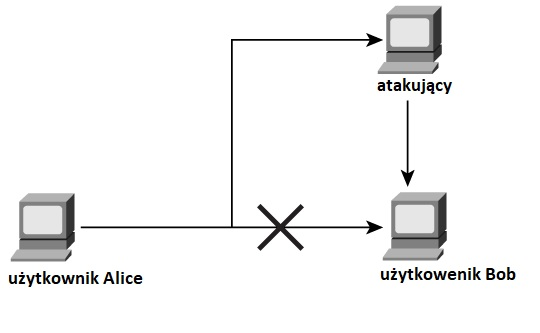
\includegraphics[width=7cm]{Powtarzajace_ataki.jpg}
\caption{Człowiek w środku - powtarzanie sesji}\label{Powtarzajace_ataki}
\end{figure}

\quad W atakach typu "porwanie sesji" atakujący dodaje się do połączenia między dwoma użytkownikami w celu przejęcia komunikacji między nimi. Na rysunku poniżej pokazano schematycznie atak typu "porwanie sesji". Użytkownik Alice wysyła wiadomość do użytkownika Bob, jednak na drodze odczytuje ją atakujący, który przez Alice jest traktowany jako użytkownik Bob. Następnie atakujący przesyła wiadomość do prawdziwego Boba i po otrzymaniu jego odpowiedzi przesyła ją do użytkownika Alice po zmodyfikowaniu. Atakujący dołącza się do połączeń w celu znalezienie luk z zabezpieczeniach. Na rys.~\ref{Porwanie_sesji} przedstawiono schemat ataku typu człowiek w środku - porwanie sesji.
\begin{figure}[H]
\centering
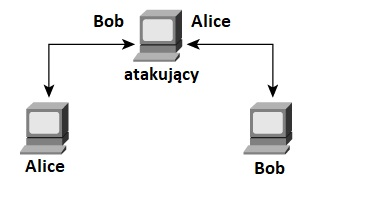
\includegraphics[width=8cm]{Porwanie_sesji.jpg}
\caption{Człowiek w środku - porwanie sesji}\label{Porwanie_sesji}
\end{figure}

\quad Prywatna wirtualna sieć zapewnia trzy etapy chroniące nas przed niepożądanymi atakami w wystarczający sposób. Pierwszym z nich jest uwierzytelnienie urządzenia, które chroni przed przechwytywaniem pakietów przez zamaskowane urządzenia atakujące. Następnym krokiem jest sprawdzenie integralności pakietów np. przy użyciu funkcji haszujących. Trzecim etapem jest zaszyfrowanie pakietów, co znacznie utrudnia przechwycenie rzeczywistych informacji ~\cite{man_in_the_middle}.
\end{description}


%\subsection{Maszyna Enigma}

\subsection{Szyfry blokowe i strumieniowe}
\subsubsection{Szyfry blokowe} 
\quad Szyfry blokowe wykorzystywane są do szyfrowania i deszyfrowania. Danymi wejściowymi do szyfrowania jest blok danych, który przy użyciu klucza szyfrującego jest przekształcany w zaszyfrowany blok danych. Odszyfrowywanie przebiega w odwrotny sposób, zaszyfrowana blokowa wiadomość przy użyciu klucza jest transformowana do odszyfrowanej blokowej wiadomości. Szyfr blokowy jest bezpieczny do momentu, kiedy klucz szyfrujący pozostaje tajny. Bez znajomości klucza niemożliwe staje się rozszyfrowanie wiadomości w satysfakcjonującym nas czasie. Im bardziej klucz jest przypadkowy tym ciężej złamać algorytm. Ważnymi parametrami szyfru blokowego jest rozmiar bloku i klucza, od których to zależy bezpieczeństwo algorytmu. Powszechnie stosowanymi rozmiarami bloków są 64 i 128 bitowe bloki, zazwyczaj algorytm DES ma 64 bitowy blok danych, zaś AES 128 bitowy blok. Długość zaszyfrowanego bloku musi być optymalna. Im większe bloki danych tym dłuższy zaszyfrowany tekst oraz większe użycie pamięci. Przy szyfrowaniu wiadomości, która ma długość 8 bitową, zaś blok szyfru ma długość 64 bity, najpierw 8 bitowa wiadomość zostanie przekonwertowana na 64 bitowy blok. Następnie 64 bitowa wiadomość zostanie zaszyfrowana przy użyciu algorytmu tworząc zaszyfrowany tekst. Do przetworzenia szyfru blokowego o rozmiarze 64 bitów potrzebujemy 64 bitów pamięci w rejestrach procesora. W dzisiejszych czasach procesory z pamięcią 64 bitową nie są kosztowne, lecz im większy chcemy utworzyć blok szyfrowy tym lepszy procesor potrzebujemy, co może mieć znaczny wpływ na wysokie koszty ~\cite{blok_cipher}.

\subsubsection{Szyfry strumieniowe}
\quad Szyfrowanie strumieniowe jest deterministyczne, co oznacza, że przy jednakowych danych wejściowych otrzymujemy taki sam wynik wyjściowy. Dzięki determinizmowi możliwe jest odszyfrowanie zaszyfrowanych strumieni bitów. Szyfrowanie strumieniowe jest podobne w działaniu do deterministycznego generatora liczb pseudolosowych, z tą różnicą że szyfrowanie strumieniowe oprócz wartości wejściowej pobiera dodatkowo klucz, który zazwyczaj ma 128 lub 256 bitów długości. Szyfrowanie strumieniowe polega na przekształceniu tekstu jawnego bit po bicie na szyfrogram. Elementy tworzące szyfrowanie strumieniowe to generator strumienia bitowy oraz element dodający np. operacja XOR. 
Operację XOR-owania przedstawiono w tabeli~\ref{xor}.

\begin{table}[H]
\centering
\begin{tabular}{|r|c|l|}
\hline
p & q & p $\veebar$ q \\
\hline
0 & 0 & \multicolumn{1}{|c|}{0} \\
\hline
0 & 1 & \multicolumn{1}{|c|}{1} \\
\hline
1 & 0 & \multicolumn{1}{|c|}{1} \\
\hline
1 & 1 & \multicolumn{1}{|c|}{0} \\
\hline
\end{tabular}
\caption{Tablica dla operacji XOR.}\label{xor}
\end{table}

Proces XOR-owania przebiega następująco:
\begin{itemize}
\item wiadomość jako tekst jawny \newline
\begin{center}
01001101
\end{center}
\item strumień klucza wytworzony przez generator strumienia klucza \newline
\begin{center}
00111000
\end{center}
\item XOR-owana wiadomość (szyfrogram) \newline
\begin{center}
01110101
\end{center}
\end{itemize}
Szyfrowanie strumieniowe polega na operacji xor tekstu jawnego(P) ze strumieniem klucza(KS) w wyniku czego otrzymano zaszyfrowaną wiadomość(C).\newline
\begin{center}
C = P $\oplus$ KS
\end{center}
Proces deszyfrowania strumieniowego polega na operacji xor tekstu zaszyfrowanego(C) z strumieniem klucza(KS), w wyniku czego otrzymano tekst jawny(P) ~\cite{stream_cipher}.\newline
\begin{center}
P = C $\oplus$ KS
\end{center}

\subsection{Szyfry symetryczne i asymetryczne}

\subsubsection{Szyfry symetryczne}
\quad Do szyfrów symetrycznych zaliczamy zarówno szyfry blokowe jak i strumieniowe. Szyfrowanie symetryczne używa jednego tajnego klucza do szyfrowania i odszyfrowywania wiadomości. W celu zaszyfrowania tekstu jawnego przy użyciu tajnego klucza szyfrujemy wiadomość do postaci tekstu zaszyfrowanego. Proces odszyfrowywania polega na przekształceniu tekstu zaszyfrowanego przy użyciu klucza w tekst jawny. Klucz jest taki sam dla procesu szyfrowania i odszyfrowywania. Do szyfrów symetrycznych zaliczamy algorytm DES, więc w jego przypadku w bloku szyfrującym będą m.in. bramki XOR. Zaś w przypadku szyfru Cezara, który też jest szyfrem symetrycznym, bramki XOR nie występują w bloku szyfrującym. Algorytm Cezara wykorzystuje metodykę przesunięcia. W szyfrach symetrycznych korzystamy z jednego klucza do szyfrowania i odszyfrowywania, w związku z czym szyfrowanie symetryczne jest prostsze niż asymetryczne, gdzie wykorzystujemy klucz publiczny i klucz prywatny. Do szyfrów symetrycznych zaliczamy:


\paragraph{1. szyfr Cezara}
\quad 

Przed erą urządzeń obliczających używano szyfry klasyczne, które działały na literach, a nie na bitach. Do szyfrów klasycznych zaliczamy słynny szyfr Cezara. Szyfr Cezara zawdzięcza swoją nazwę Juliuszowi Cezarowi, który to już w czasach starożytnych był wykorzystywany przez Juliusza. Szyfr służył do szyfrowania wiadomości poprzez zastąpienie litery literą o 3 miejsca przesuniętą względem wartości początkowej np. literę A zastąpiono literą C. W tabeli~\ref{cezar} ukazano obrazowo podstawienie z przesunięciem o trzy litery.

\begin{table}[H]
\centering
\begin{tabular}{|c|c|c|c|c|c|c|c|c|c|c|c|c|c|c|c|c|c|}
\hline
podstawa & A & Ą & B & C & Ć & D & E & Ę & F & G & H & I & J & K & L & Ł & M \\
\hline 
\hline
podstawienie & C & Ć & D & E & Ę & F & G & H & I & J & K & L & Ł & M & N & Ń & O \\
\hline
\hline
podstawa & N & Ń & O & Ó & P & R & S & Ś & T & U & W & X & Y & Z & Ż & Ź & \\
\hline 
\hline
podstawienie & Ó & P & R & S & Ś & T & U & W & X & Y & Z & Ż & Ź & A & Ą & B & \\
\hline
\end{tabular}
\caption{Szyfr Cezara z przesunięciem o trzy litery.}~\label{cezar}
\end{table}

Szyfr ten nie zapewnia bezpieczeństwa, gdyż bez problemu i w krótkim czasie można przetestować wszystkie możliwe 33 opcje w przypadku języka polskiego. Szyfr ten uniemożliwia natychmiastowe zinterpretowanie wysyłanej wiadomości po jej ujrzeniu. 

\paragraph{2. standard szyfrowania danych DES}\mbox{} \\

Algorytm zwany standardem szyfrowania danych (ang. Data Encryption Standard DES) został opatentowany przez firmę IBM i rozpowszechniony w latach siedemdziesiątych do ogólnego użytku, początkowo miał nazwę Lucyfer. We wczesnych latach siedemdziesiątych nie znane były nikomu algorytmy szyfrowania do momentu opatentowania przez firmę IBM algorytmu DES i jego rozpowszechnienia. Standard szyfrowania danych jest szyfrem blokowym, co znaczy, że dane są dzielone na bloki o długości 64 bitów i następnie szyfrowane. Danymi wejściowymi algorytmu jest blok tekstu jawnego o długości 64 bitów, który po przetworzeniu przez algorytm przedstawiono jako szyfrogram. Długość klucza w 64 bitowym bloku wynosi 56 bitów, gdzie co ósmy bit jest bitem parzystości. Algorytm DES składa się z 16 cykli, które są wykonywane jeden po drugim. Algorytm można podzielić na poszczególne kroki:

\begin{itemize}
\item zamiana 64 bitowego klucza decymalnego na postać binarną i usunięcie co ósmego bitu zwanego bitem parzystości, w wyniku czego otrzymano 56 bitowy binarny klucz,
\item permutacja 56 bitowego klucza binarnego zgodnie z tabelą~\ref{per_klucza} dla każdego z 16 cykli,
\item podział 56 bitowego klucza na prawą o lewą część o długości 28 bitów i przesunięcie bitowe, które jest zależne od cyklu co ukazuje tabela~\ref{przesuniecie_klucza},
\item permutacja kompresji klucza DES zgodnie z tabelą~\ref{per_kompresji} kompresująca klucz 56 bitowy do klucza 48 bitowego dla każdego z 16 cykli ukazanego na rysunku~\ref{des} jako $K_{i}$,
\item zamiana wiadomości tekstowej na wiadomość w postaci heksadecymalnej i binarnej,
\item transpozycja wiadomości binarnej z tabelą permutacji początkowej,
\item podział wiadomości 64 bitowej na dwie części 32 bitowe: strona prawa oznaczona literą P na rysunku~\ref{des} i strona lewa oznaczona literą L na rysunku~\ref{des},
\item prawa cześć wiadomości ulega rozszerzeniu zgodnie z tabelą~\ref{per_rozszerzenia} permutacji rozszerzenia, w wyniku czego otrzymano 48 bitową wiadomość,
\item operacja XOR obliczonego klucza dla danej rundy z 48 bitową wiadomością otrzymaną w wyniku permutacji rozszerzenia,
\item transpozycja wyniku operacji XOR z tablicą S bloków na rysunku~\ref{des} oznaczono S-boxes,
\item wyjście S bloku ulega transpozycji z tabelą permutacji bloku P na rysunku~\ref{des} oznaczono jako P box,
\item wiadomość po permutacji bloku P poddano operacji XOR z lewą częścią wiadomości, w wyniku czego otrzymano 32 bitową część prawą wiadomości,
\item lewą częścią 32 bitowej wiadomości jest prawa część 32 bitowej wiadomości bez żadnych zmian.
\end{itemize}
Dane wyjściowe wiadomości z rundy pierwszej są danymi wejściowymi dla rundy drugiej algorytmu. Kroki przedstawione powyżej należy wykonać 16 razy w calu zaszyfrowania wiadomości, która jest podzielona na bloki 64 bitowe. Na obrazku~\ref{des} zobrazowano pojedynczą rundę algorytmu DES.

\begin{figure}[H]
\centering
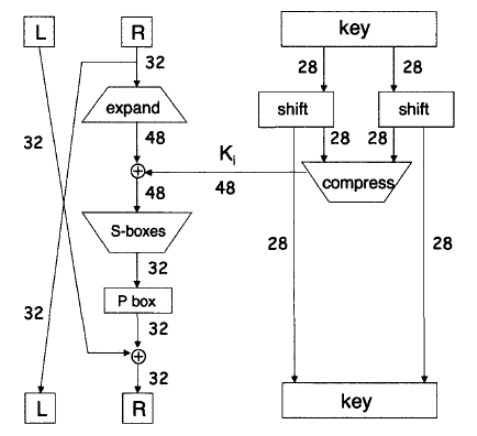
\includegraphics{des}
\caption{Pojedyncza runda algorytmu DES ~\cite{DES}.
}\label{des}
\end{figure}

W tabeli~\ref{hex_to_bin} ukazano reprezentację binarną liczą heksadecymalnych w systemie 64 bitowym.

\begin{table}[H]
\centering
\begin{tabular}{|c|c|c|c|c|c|c|c|c|}
\hline
0 & 1 & 2 & 3 & 4 & 5 & 6 & 7\\
\hline
0000 & 0001 & 0010 & 0011 & 0100 & 0101 & 0110 & 0111\\
\hline
8 & 9 & A & B & C & D & E & F\\
\hline
1000 & 1001 & 1010 & 1011 & 1100 & 1101 & 1110 & 1111\\
\hline
\end{tabular}
\caption{Reprezentacja binarna liczb heksadecymalnych.}~\label{hex_to_bin}
\end{table}
\newpage
W tabeli~\ref{per_poczatkowa} przedstawiono tablicę dla permutacji początkowej wiadomości dla algorytmu DES. Permutacji dokonuje się poprzez zamianę miejscami bitów zgodnie z tabelą permutacji otrzymując w wyniku przekształcone dane wejściowe.

\begin{table}[H]
\centering
\begin{tabular}{|c|c|c|c|c|c|c|c|c|c|c|c|c|c|c|c|}
\hline
58 & 50 & 42 & 34 & 26 & 18 & 10 & 2 & 60 & 52 & 44 & 36 & 28 & 20 & 12 & 4\\
\hline
62 & 54 & 46 & 38 & 30 & 22 & 14 & 6 & 64 & 56 & 48 & 40 & 32 & 24 & 16 & 8\\
\hline
57 & 49 & 41 & 33 & 25 & 17 & 9 & 1 & 59 & 51 & 43 & 35 & 27 & 19 & 11 & 3\\
\hline
61 & 53 & 45 & 37 & 29 & 21 & 13 & 5 & 63 & 55 & 47 & 39 & 31 & 23 & 15 & 7\\
\hline
\end{tabular}
\caption{Permutacja początkowa DES.}\label{per_poczatkowa}
\end{table}

Tabela~\ref{per_klucza} ukazuje permutacje klucza 56 bitowego, który powstaje z klucza 64 bitowego w wyniku usunięcia co ósmego bitu parzystości.%Czemu usuwamy bit parzystości?

\begin{table}[H]
\centering
\begin{tabular}{|c|c|c|c|c|c|c|c|c|c|c|c|c|c|}
\hline
57 & 49 & 41 & 33 & 25 & 17 & 9 & 1 & 58 & 50 & 42 & 34 & 26 & 18\\
\hline
10 & 2 & 59 & 51 & 43 & 35 & 27 & 19 & 11 & 3 & 60 & 52 & 44 & 36\\
\hline
63 & 55 & 47 & 39 & 31 & 23 & 15 & 7 & 62 & 54 & 46 & 38 & 30 & 22\\
\hline
14 & 6 & 61 & 53 & 45 & 37 & 29 & 21 & 13 & 5 & 28 & 20 & 12 & 4 \\
\hline
\end{tabular}
\caption{Permutacja klucza DES.}~\label{per_klucza}
\end{table}
 
Przesunięcia bitowe dwóch kluczy 28 bitowych tworzących wejściowy klucz 56 bitowy dla każdego cyklu zależą od numeru cyklu, co ukazano w tabeli~\ref{przesuniecie_klucza}.

\begin{table}[H]
\begin{tabular}{|c|c|c|c|c|c|c|c|c|c|c|c|c|c|c|c|c|}
\hline
cykl&1&2&3&4&5&6&7&8&9&10&11&12&13&14&15&16\\
\hline
liczba przesunięć&1&1&2&2&2&2&2&2&1&2&2&2&2&2&2&1\\ \hline
\end{tabular}
\caption{Liczba przesunięć klucza w zależności od cyklu dla algorytmu DES.}\label{przesuniecie_klucza}
\end{table} 
 
Po operacji przesunięcia bitowego klucza 56 bitowego wykonano kompresję klucza do rozmiaru 48 bitów zgodnie z tabelą~\ref{per_kompresji}.
 
\begin{table}[H]
\centering
\begin{tabular}{|c|c|c|c|c|c|c|c|c|c|c|c|}
\hline
14 & 17 & 11 & 24 & 1 & 5 & 3 & 28 & 15 & 6 & 21 & 10\\
\hline
23 & 19 & 12 & 4 & 26 & 8 & 16 & 7 & 27 & 20 & 13 & 2\\
\hline
41 & 52 & 31 & 37 & 47 & 55 & 30 & 40 & 51 & 45 & 33 & 48\\
\hline
44 & 49 & 39 & 56 & 34 & 53 & 46 & 42 & 50 & 36 & 29 & 32\\
\hline
\end{tabular}
\caption{Permutacja kompresji DES.}~\label{per_kompresji}
\end{table}
\newpage
Tabela~\ref{per_rozszerzenia} jest stosowana do operacji rozszerzenia wiadomości. Wiadomość 64 bitowa zostaje podzielona na dwa 32 bitowe bloki, które następnie ulegają rozszerzeniu do dwóch 48 bitowych bloków zgodnie z tabelą~\ref{per_rozszerzenia} permutacji rozszerzenia. Rozszerzone 48 bitowe bloki zawierają powtórzenia bitów, rozszerzenie 32 do 48 bitów powoduje wystąpienie 16 bitów, które nie są unikatowe. Oznacza to, że 8 bitów występuje podwójnie w szyfrowanej wiadomości.

\begin{table}[H]
\centering
\begin{tabular}{|c|c|c|c|c|c|c|c|c|c|c|c|}
\hline
32 & 1 & 2 & 3 & 4 & 5 & 4 & 5 & 6 & 7 & 8 & 9\\
\hline
8 & 9 & 10 & 11 & 12 & 13 & 12 & 13 & 14 & 15 & 16 & 17\\
\hline
16 & 17 & 18 & 19 & 20 & 21 & 20 & 21 & 22 & 23 & 24 & 25\\
\hline
24 & 25 & 26 & 27 & 28 & 29 & 28 & 29 & 30 & 31 & 32 & 1\\
\hline
\end{tabular}
\caption{Permutacja rozszerzenia DES.}~\label{per_rozszerzenia}
\end{table}

Po dokonaniu permutacji rozszerzenia wiadomości dokonano operacji xor otrzymanej wiadomości z obliczonym kluczem dla danego cyklu. Otrzymany wynik podzielono na 8 bloków 6 bitowych, które wykorzystano do dalszych obliczeń z pomocą tabeli~\ref{s_bloki} struktury S bloków. Z każdego bloku 6 bitowego odczytano wartość pierwszego i ostatniego bitu, wartość 00 oznacza wykorzystanie wiersza pierwszego z danego bloku, 01 oznacza wiersz drugi, 10 oznacza wiersz trzeci, natomiast 11 oznacza wiersz czwarty. Wartości od bita drugiego do piątego zamieniamy na postać heksadecymalną i odczytujemy dla niej wartość z danego bloku np. jeśli pierwszy i ostatni bit to 00 to wartość odczytano z wiersza pierwszego, gdy bity między 2-5 pozycją to 1111 oznacza to ostatnią wartość z wiersza pierwszego czyli 7.

\begin{table}[H]
\centering
\begin{adjustbox}{width=0.8\textwidth}
\begin{tabular}{|c|c|c|c|c|c|c|c|c|c|c|c|c|c|c|c|c|}
\hline
\multicolumn{16}{|c|}{S blok 1}\\ 
\hline
14&4&13&1&2&15&11&8&3&10&6&12&5&9&0&7 \\ \hline
0 &	15& 	7 &	4 &	14 &	2& 	13& 	1 &	10 &	6 &	12 &	11 &	9 &	5 &	3 &	8 \\ \hline
4 &	1 &	14 &	8 	&13 	&6 &	2& 	11& 	15& 	12 &	9 	&7& 	3& 	10& 	5& 	0 \\ \hline
15 &	12& 	8 &	2 &	4 &	9 &	1 &	7 &	5 &	11 &	3 &	14 &	10 &	0 &	6 &	13 \\ \hline
\multicolumn{16}{|c|}{S blok 2} \\ \hline
15 &	1 &	8 &	14 &	6 &	11 &	3 &	4 &	9 &	7 &	2 &	13 &	12 &	0 &	5 &	10 \\ \hline
3 &	13& 	4 &	7 &	15 &	2 &	8 &	14 &	12 &	0 &	1 &	10 &	6 &	9 &	11 &	5 \\ \hline
0 &	14 &	7 &	11 &	10 &	4 &	13 &	1 &	5 &	8 &	12 &	6 &	9 &	3 &	2 &	15 \\ \hline
13 &	8 &	10 &	1 &	3 &	15 &	4 &	2 &	11 &	6 &	7 &	12 &	0 &	5 &	14 &	9 \\ \hline
\multicolumn{16}{|c|}{S blok 3}\\ \hline
10 &	0 &	9 &	14 &	6 &	3 &	15 &	5 &	1 &	13 &	12 &	7 &	11 &	4 &	2 &	8\\ \hline
13 &	7 &	0 &	9 &	3 &	4 &	6 &	10 &	2 &	8 &	5 &	14 &	12 &	11 &	15 &	1\\ \hline
13 &	6 &	4 &	9 &	8 &	15 &	3 &	0 &	11 &	1 &	2 &	12 &	5 &	10 &	14 &	7\\ \hline
1 &	10 &	13 &	0 &	6 &	9 &	8 &	7 &	4 &	15 &	14 &	3 &	11 &	5 &	2 &	12 \\ \hline
\multicolumn{16}{|c|}{S blok 4}\\ \hline
7 &	13 &	14 &	3 &	0 &	6 &	9 &	10 &	1 &	2& 	8& 	5& 	11& 	12& 	4& 	15\\ \hline
13& 	8& 	11& 	5& 	6& 	15& 	0& 	3& 	4& 	7& 	2& 	12& 	1& 	10& 	14& 	9\\ \hline
10& 	6& 	9& 	0& 	12& 	11& 	7& 	13& 	15& 	1& 	3& 	14& 	5& 	2& 	8& 	4\\ \hline
3& 	15& 	0& 	6& 	10& 	1& 	13& 	8& 	9& 	4& 	5& 	11& 	12& 	7& 	2& 	14\\ \hline
\multicolumn{16}{|c|}{S blok 5}\\ \hline
2& 	12& 	4& 	1& 	7& 	10& 	11& 	6& 	8& 	5& 	3& 	15& 	13& 	0& 	14& 	9\\ \hline
14& 	11& 	2& 	12& 	4& 	7& 	13& 	1& 	5& 	0& 	15& 	10& 	3& 	9& 	8& 	6\\ \hline
4& 	2& 	1& 	11& 	10& 	13& 	7& 	8& 	15& 	9& 	12& 	5& 	6& 	3& 	0& 	14\\ \hline
11& 	8& 	12& 	7& 	1& 	14& 	2& 	13& 	6& 	15& 	0& 	9& 	10& 	4& 	5& 	3\\ \hline 
\multicolumn{16}{|c|}{S blok 6}\\ \hline
12& 	1& 	10& 	15& 	9& 	2& 	6& 	8& 	0& 	13& 	3& 	4& 	14& 	7& 	5& 	11\\ \hline
10 &	15& 	4& 	2& 	7& 	12& 	9& 	5& 	6& 	1& 	13& 	14& 	0& 	11& 	3& 	8\\ \hline
9& 	14& 	15& 	5& 	2& 	8& 	12& 	3& 	7& 	0& 	4& 	10& 	1& 	13& 	11& 	6\\ \hline
4& 	3& 	2& 	12& 	9& 	5& 	15& 	10& 	11& 	14& 	1& 	7& 	6& 	0& 	8& 	13\\ \hline
\multicolumn{16}{|c|}{S blok 7}\\ \hline
4& 	11& 	2& 	14& 	15& 	0& 	8& 	13& 	3& 	12& 	9& 	7& 	5& 	10& 	6& 	1\\ \hline
13& 	0& 	11& 	7& 	4& 	9& 	1& 	10& 	14& 	3& 	5& 	12& 	2& 	15& 	8& 	6\\ \hline
1& 	4& 	11& 	13& 	12& 	3& 	7& 	14& 	10& 	15& 	6& 	8& 	0& 	5& 	9& 	2\\ \hline
6& 	11& 	13& 	8& 	1& 	4& 	10& 	7& 	9& 	5& 	0& 	15& 	14& 	2& 	3& 	12\\ \hline 
\multicolumn{16}{|c|}{S blok 8}\\ \hline
13& 	2& 	8& 	4& 	6& 	15& 	11& 	1& 	10& 	9& 	3& 	14& 	5& 	0& 	12& 	7\\ \hline
1& 	15& 	13& 	8& 	10& 	3& 	7& 	4& 	12& 	5& 	6& 	11& 	0& 	14& 	9& 	2\\ \hline
7& 	11& 	4& 	1& 	9& 	12& 	14& 	2& 	0& 	6& 	10& 	13& 	15& 	3& 	5& 	8\\ \hline
2& 	1& 	14& 	7& 	4& 	10& 	8& 	13& 	15& 	12& 	9& 	0& 	3& 	5& 	6& 	11 \\ \hline
\end{tabular}
\end{adjustbox}
\caption{Struktury S bloków algorytmu DES.}\label{s_bloki}
\end{table}



\begin{table}[H]
\centering
\begin{tabular}{|c|c|c|c|c|c|c|c|c|}
\hline
16 &	7 &	20& 	21& 	29& 	12& 	28& 	17\\ \hline
1 &	15& 	23& 	26& 	5& 	18& 	31& 	10\\ \hline
2 &	8 &	24 &	14& 	32& 	27& 	3 &	9\\ \hline
19 	&13 &	30& 	6& 	22& 	11& 	4& 	25\\ \hline
\end{tabular}
\caption{Permutacja bloku P algorytmu DES.}~\label{blok_P}
\end{table}

Algorytm DES nie jest obecnie uznawany za bezpieczny przez Amerykańskie Standardy Federalne. W roku 2015 przy użyciu wysokiej wydajności FPGA możliwe było złamanie szyfru w stosunkowo krótkim czasie(4-5 dni). Dla atakujących przestała być odstraszająca cena platformy FPGA w porównaniu do zysków jakie może dać im atak. W celu przesłania klucza do drugiej osoby, z którą tworzymy bezpieczne połączenie wymagane jest znalezienie bezpiecznej metody przesyłania klucza. Zaletami algorytmu DES jest jego odporność na błędy, dzięki jego prostocie. W obecnych czasach jest on nadal popularny w użytku, dzięki swojej szybkości ~\cite{DES}.

%%% cos o deszyfracji dodac

%\paragraph{AES} \mbox{} \\


\paragraph{3. międzynarodowy algorytm szyfrowania danych IDEA} \mbox{} \\ 

IDEA to Międzynarodowy Algorytm Szyfrowania Danych(z ang. International Data Encryption Algorithm). Początkowo nosił nazwę PES(z ang. Proposed Encryption Standard) został opatentowany przez Xuejia Lai i Jamesa Massey w 1990 roku. Następnie został on ulepszony przed atakiem zmieniając nazwę na IPES(z ang.Improved Proposed Encryption Standard). Ostatecznie jego nazwę zmieniono na obecnie używaną IDEA w 1992 roku. Jest to algorytm blokowy, który wykorzystuje bloki 64 bitowe i klucz o długości 128 bitów. Do szyfrowania i odszyfrowywania wykorzystuje się ten sam algorytm. Algorytm ten początkowo dzieli blok 64 bitowy na 4 pod bloki 16 bitowe, na których dokonywane są operację: XOR, dodawanie modulo i mnożenie modulo. Algorytm składa się z ośmiu rund. Na rysunku~\ref{idea} przedstawiono pojedyncza rundę algorytmu IDEA, gdzie pierwsza 16 bitowa część wiadomości podlega operacji mnożenia modulo z 16 bitowym kluczem rundy. Operacja modulo oznaczona przy pomocy kółka z kropką w środku $\odot$. Druga 16 bitowa część wiadomości poddano operacji dodawania modulo z 16 bitowym kluczem rundy. Operacje dodawania modulo oznaczono kwadratem z plusem w środku $\boxplus$. Operację XOR oznaczono okręgiem z plusem w środku $\oplus$. Operacje mnożenia, dodawania i xorowania są wykonywane na częściach wiadomości zgodnie z rysunkiem~\ref{idea}. Po operacjach xorowania, dodawania i mnożenia dokonujemy przestawienia bloku drugiego z trzecim, które są danymi wejściowymi do następnej rundy. W każdej rundzie używany jest 16 bitowy klucz dla danego podbloku. Po zakończeniu ośmiu rund, cztery bloki są złożone do jednego bloku 64 bitowego, który jest wynikiem końcowym.

\begin{figure}[H]
\centering
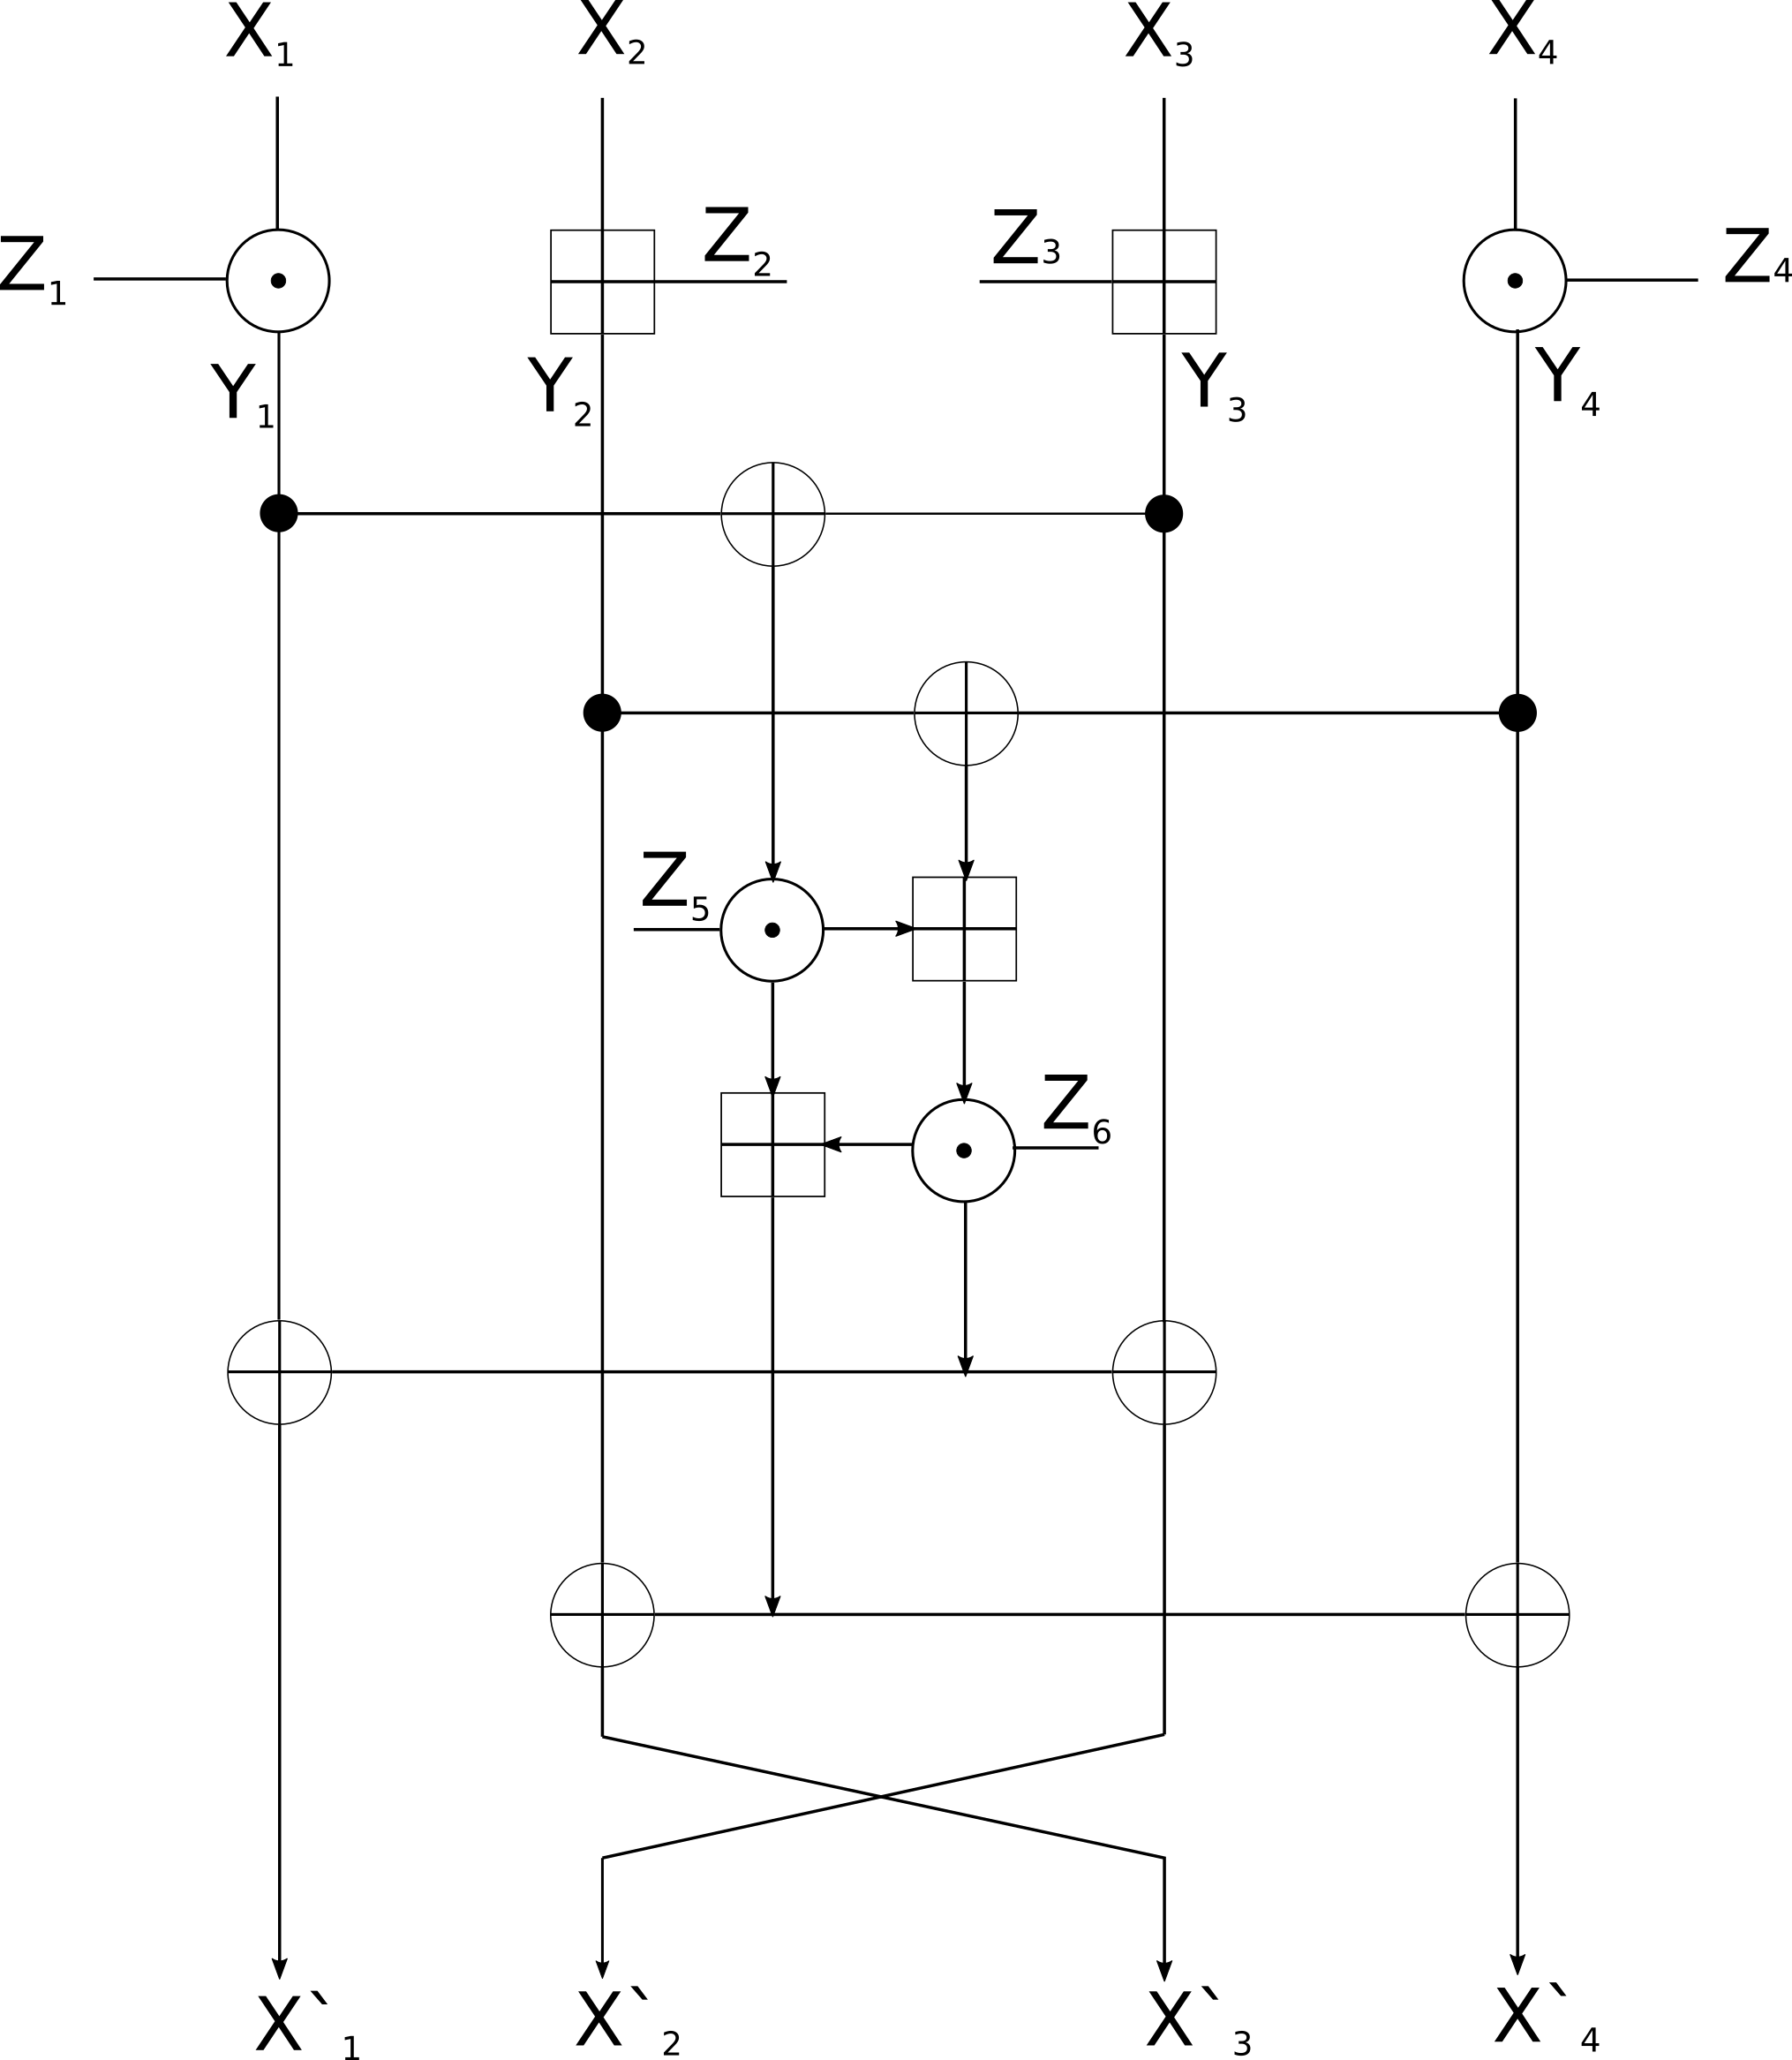
\includegraphics[width=7cm]{idea.png}
\caption{Pojedyncza runda algorytmu IDEA ~\cite{IDEA}.}\label{idea}
\end{figure}


Dla operacji dodawania modulo potrzebne są dwie liczby, na których zostanie wykonane działanie oraz tzn. licza modulo. Operacja dodawania modulo przebiega w następujących krokach: dodanie do siebie dwóch liczb, a następnie podzielenie wyniku dodawania przez liczbę modulo. Reszta z wyniku dzielenia sumy dwóch liczb przez liczbę module daje nam wynik operacji dodawania modulo. Operacje dodawania modulo oznaczono symbolem $\boxplus$. Przykładem operacji dodawania modulo jest: 2 $\boxplus$ 5 $\equiv$ 1 (mod 3). Dla operacji mnożenia modulo potrzebne są dwie liczby, na których zostanie wykonane działanie oraz tzn. liczba modulo. Operacja mnożenia modulo polega na iloczynie dwóch czynników oraz ilorazie wyniku operacji z liczbą modulo. Wynikiem jest reszta z operaji dzielenia przez liczbę modulo. Operacje mnożenia modulo oznaczono symbolem $\odot$. Przykładem operacji mnożenia modulo jest 2  $\odot$ 7 = 2 (mod 3), bo 2*7 = 14, gdzie 14/3 daje resztę z dzielenia 2.
Klucz o długości 128 bitów jest dzielony na osiem 16 bitowych podkluczy. Dla każdej rundy zostaje wykorzystane 6 podkluczy, które oznaczono na rysunku~\ref{idea} literą Z. Do wszystkich rund, których jest 8 użyto 52 podkluczy oraz 4 podklucze użyte do końcowych przekształceń. Dla algorytmu IDEA użyto łącznie 52 podkluczy, które stworzono z 128 bitowego klucza. Generację klucza 128 bitowego do 52 podkluczy można podzielić na:
\begin{itemize}
\item podział 128 bitowego klucza na 8 podkluczy 16 bitowych, gdzie pierwsze 6 podkluczy wykorzystano do rundy 1, a następne 2 podklucze użyto do rundy 2 algorytmu
\item przesunięcie klucza 128 bitowego w lewo o 25 bitów i ponowny podział na 8 podkluczy, gdzie pierwsze 4 podklucze użyto do rundy drugiej, a następne 4 podklucze wykorzystano w rundzie 3
\item klucz jest dalej analogicznie przesuwany i dzielony, aż do momentu uzyskania 52 podkluczy
\end{itemize}

Proces deszyfrowania wiadomości również korzysta z schematu przedstawionego na rysunku~\ref{idea} pojedynczej rundy algorytmu, składa się on również z 8 rund. Proces tworzenia podkluczy z klucza odbywa się na podstawie podkluczy wykorzystanych do zaszyfrowania wiadomości. Przy utworzeniu klucza pomocna jest tabela multiplikatywnej odwrotności 4 bitowej liczby binarnej przedstawionej w tabeli~\ref{nibel}.

\begin{table}[H]
\centering
\begin{tabular}{|c|c|c|}
\hline
\thead{wartość \\ binarna[decymalna]} & \thead{multiplikatywna \\  odwrotność[decymalna]} & \thead{addytywna \\ odwrotność[decymalna]}\\ \hline
0000 [0]&0000 [0]&0000 [0] \\ \hline
 0001 [1]&1111 [15]&0001 [1]\\ \hline
 0010 [2]&1110 [14]&1001 [9]\\ \hline
 0011 [3]&1101 [13]&0110 [6]\\ \hline
 0100 [4]&1100 [12]&1101 [13]\\ \hline
 0101 [5]&1011 [11]&0111 [7]\\ \hline
 0110 [6]&1010 [10]&0011 [3]\\ \hline
 0111 [7]&1001 [9]&0101 [5]\\ \hline
 1000 [8]&1000 [8]&1111 [15]\\ \hline
 1001 [9]&0111 [7]&0010 [2]\\ \hline
 1010 [10]&0110 [6]&1100 [12]\\ \hline
 1011 [11]&0101 [5]&1110 [14]\\ \hline
 1100 [12]&0100 [4]&1010 [10]\\ \hline
 1101 [13]&0011 [3]&0100 [4]\\ \hline
 1110 [14]&0010 [2]&1011 [11]\\ \hline
 1111 [15]&0001 [1]&1000 [8]\\ \hline
 \end{tabular}
\caption{Obliczenia multiplikatywnej i addytywnej odwrotności ~\cite{IDEAA}.}\label{nibel}
\end{table}

Multiplikatywną odwrotność dla a wyliczono według zależności x mod n, gdzie a $\in$ $Z_{n}$ oraz n jest rozmiarem grupy. Do obliczenia odwrotności addytywnej wykorzystano rozszerzony algorytm Euklidesa, który oblicza liczby całkowite x i y wykorzystując zależność ax + ny = 1, gdzie a $\in$ $Z_{n}$. Proces tworzenia podkluczy wykorzystanych do deszyfrowania ukazano w tabeli~\ref{podklucze_deszyfrowania_idea}. Potęga oznaczona literą a określa multiplikatywną odwrotność danej liczby, potęga oznaczona jako m określa addytywną odwrotność podanej liczby.
% opisac addytywna odwrotnosc i dlaczego 0


\begin{table}[H]
\centering
\begin{tabular}{|c|c|c|c|c|c|c|c|c|c|c|c|c|}
\hline
cykl & \multicolumn{6}{|c|}{podklucze szyfrujące}  & \multicolumn{6}{|c|}{podklucze deszyfrujące} \\ \hline
1&$x_{1}$&$x_{2}$&$x_{3}$&$x_{4}$&$x_{5}$&$x_{6}$&$x_{49}^{a}$&$x_{50}^{m}$&$x_{51}^{m}$&$x_{52}^{a}$&$x_{47}$&$x_{48}$\\ \hline
2&$x_{7}$&$x_{8}$&$x_{9}$&$x_{10}$&$x_{11}$& $x_{12}$&$x_{43}^{a}$&$x_{45}^{m}$&$x_{44}^{m}$&$x_{46}^{a}$&$x_{41}$&$x_{42}$\\ \hline
3&$x_{13}$&$x_{14}$&$x_{15}$&$x_{16}$&$x_{17}$&$x_{18}$&$x_{37}^{a}$&$x_{39}^{m}$&$x_{38}^{m}$&$x_{40}^{a}$&$x_{35}$&$x_{36}$\\ \hline
4&$x_{19}$&$x_{20}$&$x_{21}$&$x_{22}$&$x_{23}$&$x_{24}$&$x_{31}^{a}$&$x_{33}^{m}$&$x_{32}^{m}$&$x_{34}^{a}$&$x_{29}$&$x_{30}$\\ \hline
5&$x_{25}$&$x_{26}$&$x_{27}$&$x_{28}$&$x_{29}$&$x_{30}$&$x_{25}^{a}$&$x_{27}^{m}$&$x_{26}^{m}$&$x_{28}^{a}$&$x_{23}$&$x_{24}$\\ \hline
6&$x_{31}$&$x_{32}$&$x_{33}$&$x_{34}$&$x_{35}$&$x_{36}$&$x_{19}^{a}$&$x_{21}^{m}$&$x_{20}^{m}$&$x_{22}^{a}$&$x_{17}$&$x_{18}$\\ \hline
7&$x_{37}$&$x_{38}$&$x_{39}$&$x_{40}$&$x_{41}$&$x_{42}$&$x_{13}^{a}$&$x_{15}^{m}$&$x_{14}^{m}$&$x_{16}^{a}$&$x_{11}$&$x_{12}$\\ \hline
8&$x_{43}$&$x_{44}$&$x_{45}$&$x_{46}$&$x_{47}$&$x_{48}$&$x_{7}^{a}$&$x_{9}^{m}$&$x_{8}^{m}$&$x_{10}^{a}$&$x_{5}$&$x_{6}$\\ \hline
dodatkowe 4 podklucze&$x_{49}$&$x_{50}$&$x_{51}$&$x_{52}$&&&$x_{1}^{a}$&$x_{2}^{m}$&$x_{3}^{m}$&$x_{4}^{a}$&&\\ \hline
\end{tabular}
\caption{Podklucze szyfrujące i deszyfrujące IDEA.}\label{podklucze_deszyfrowania_idea}
\end{table}

Jedną z podstawowych zalet algorytmu są proste operacje na bitach tj. mnożenie i dodawanie modulo oraz xorowanie. Do szyfrowania i deszyfrowania wiadomości wykorzystuje ten sam proces, natomiast podklucze są różne dla szyfrowania i odszyfrowywania. Algorytm IDEA wolniej szyfruje dane niż algorytm DES, jednak dzięki temu, że jego klucz jest dwa razy dłuższy niż w DES ataki brutalne są mniej skuteczne ~\cite{IDEA}.

%\paragraph{Blowfish} \mbox{} \\


\subsubsection{Szyfry asymetryczne}

\quad Szyfry asymetryczne charakteryzują się tym, że posiadają osobny klucz do szyfrowania i osobny deszyfrowania. W celu wyjaśnienia zasady działania szyfru asymetrycznego przedstawiono powszechnie znany sposób wysyłania wiadomości od Alicji do Boba przedstawiony schematycznie na rysunku~\ref{rsa}.

\begin{figure}[H]
\centering
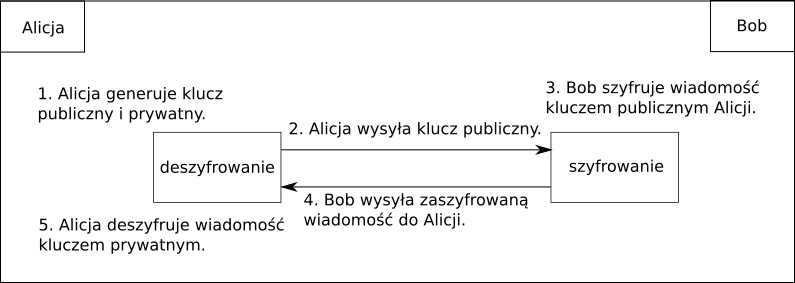
\includegraphics[width=15cm]{rsa.png}
\caption{Schematyczne szyfrowanie asymetryczne.}\label{rsa}
\end{figure}
\newpage
Do szyfrowania używany jest klucz publiczny, natomiast do odszyfrowania wiadomości użyto klucza prywatnego. Bob generuje publiczny klucz, który może być znany dla każdego, gdyż tylko Bob mający klucz prywatny może odszyfrować wiadomość zaszyfrowaną przy pomocy jego publicznego klucza. Szyfrowanie asymetryczne jest bezpieczne nawet w przypadku wystąpienia osoby trzeciej Ewy, która chciałaby podsłuchać konwersację między Bobem, a Alicją. Bob po wygenerowaniu klucza publicznego wysyła go do Alicji, aby ta mogą zaszyfrować wiadomość, którą chce do niego przesłać. W przypadku gdy Ewa przechwyci klucz publiczny Boba, nie jest w stanie odszyfrować wiadomości, gdyż nie posiada klucza prywatnego Boba, w którego posiadaniu jest tylko on. W celu przesłania wiadomości od Boba do Alicji proces wygląda tak samo. Na rysunku~\ref{rsa} zobrazowano szyfrowanie i deszyfrowanie z użyciem klucza publicznego i prywatnego. Alicja generuje klucz publiczny, który wysyła do Boba. Bob szyfruje wiadomość publicznym kluczem Alicji i przesyła jej zaszyfrowaną wiadomość, która Alicja odszyfruje przy użyciu jej klucza prywatnego. Obecność dwóch kluczy w algorytmie rozwiązuje problem wymiany klucza, co pozwala osobom będącym daleko od siebie w bezpieczny sposób się komunikować ~\cite{asymetric}. Do szyfrów asymetrycznych zaliczamy:



\paragraph{1. algorytm Rivesta-Shamira-Adlemana RSA} \mbox{} \\

Algorytm RSA jest jednym z powszechniejszym algorytmów. Algorytm RSA zawdzięcza swoją nazwę trzem osobom, przez które został on opatentowany przez Rona Rivest, Adi Shamir i Leonard Adleman w 1977 roku. Nazwa algorytmu RSA pochodzi od pierwszych liter nazwisk wynalazców. Algorytm RSA bazuje na liczbach pierwszych oraz faktoryzacji dużych liczb. Proces tworzenia pary kluczy: prywatnego i publicznego przebiega w następujących krokach:
\begin{itemize}
\item wybór dwóch odpowiednio dużych licz pierwszych, które po przemnożeniu dadzą klucz o pożądanym rozmiarze np. 2048 bitów
\begin{center}
n = p * q 
\end{center}
gdzie n to wynik mnożenia liczb pierwszych, p i q liczby pierwsze.
\item obliczenie funkcji Eulera według zależności
\begin{center}
m = (p-1)(q-1)
\end{center}
\item określenie liczby e względnie pierwszej z m oraz spełnia zależność 1<e<m
\item obliczenie liczby d według zależności
\begin{center}
d*e mod(m) = 1
\end{center}
\item obliczone liczby e i d są publiczne, natomiast liczba d jest trzymana w tajemnicy
\item zaszyfrowanie wiadomości c z wykorzystaniem wartości publicznych
\begin{center}
c = $m^{e}$mod(n)
\end{center}
\item do odszyfrowania wiadomości wykorzystano liczbę prywatną d według zależności
\begin{center}
p = $c^{d}$mod(n)
\end{center}
\end{itemize}
 
 
 
\paragraph{2. algorytm Diffie-Hellman} \mbox{} \\

Algorytm Diffie-Hellman został opatentowany w 1976 roku przez Whitfield Diffie i Martin Hellman. Dzięki temu algorytmowi możliwe jest przesyłanie klucza przez niezabezpieczone łącze w bezpieczny sposób. Obecnie jest on stosowany do wymiany klucza symetrycznego. Algorytm można opisać w następujących krokach: 
\begin{itemize}
\item Alicja generuje prywatną liczbę całkowitą a,
\item Bob generuje prywatną liczbę całkowitą b,
\item wybór liczby pierwszej p,
\item obliczenie publicznej wartości z wykorzystaniem liczby piwerszej p, wartości g oraz prywatnej liczby a (dla Alicji) i b (dla Boba) według zależności
\begin{center}
$g^{a}$mod(p) i $g^{b}$mod(p),
\end{center}
\item wymiana publicznej wartości między Alicją i Bobem,
\item Alicja oblicza
\begin{center}
$g^{ab}$ = $(g^{b})^{a}$mod(p),
\end{center}
\item Bob oblicza
\begin{center}
$g^{ba}$ = $(g^{a})^{b}$mod(p),
\end{center}
\item Alicja i Bob posiadają wspólny tajny klucz k, gdyż
\begin{center}
$g^{ab}$ = $g^{ba}$.
\end{center}
\end{itemize}

Algorytm Diffie-Hellmana przestanie być bezpieczny w momencie, gdy zostanie rozwiązany problem logarytmu dyskretnego. Wartościami publicznymi powiązanymi poniższą relacją są g, p, a i b.
\begin{center}
$g^{a}$ $\equiv$ a mod(p) oraz $g^{b}$ $\equiv$ b mod(p)
\end{center}
Obecnie nie istnieje żaden algorytm umożliwiający rozwiązanie problemu logarytmu dyskretnego ~\cite{DH}.

%\paragraph{Funkcje haszujące} \mbox{} \\
\newpage
\subsection{Protokoły}
\subsubsection{VPN with Point-to-Point Tunneling Protocol (PPTP)}
\quad Protokół punkt - punkt często wykorzystywany na urządzeniach z systemem operacyjnym Windows w celu utworzenia wirtualnej sieci prywatnej. Protokół PPTP został utworzony w czasach sieci wdzwanianej tzn. dial up, jednak bez problemu można z niego korzystać również dla sieci Ethernet, Internet czy cyfrowej sieci usług zintegrowanych(ISDN). Utworzenie sieci VPN w sieci TCP/IP umożliwia bezpieczny transfer danych między zdalnym komputerem, a serwerem. Do implementacji protokołu głównie jest wykorzystywany: klient PPTP, serwer NAS(ang. Network Attached Storage) i serwer PPTP. Serwer NAS bezpiecznie przechowuje dane i udostępnia je tylko wybranym użytkownikom. Na rys.~\ref{PPTP} poniżej poglądowo przedstawiono komunikację z użyciem protokołu PPTP. 
\begin{figure}[H]
\centering
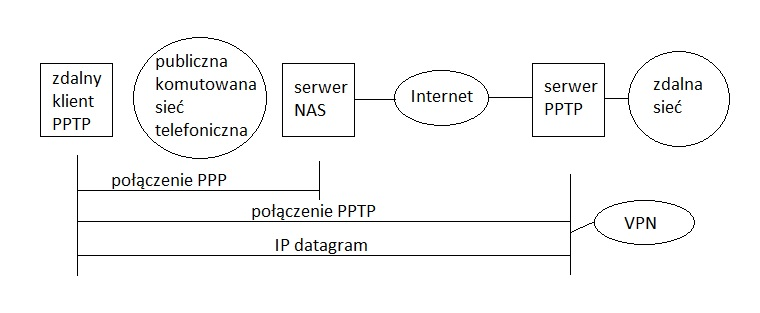
\includegraphics[width=12cm]{komunikacja_PPTP.jpg}
\caption{Poglądowa komunikacja z użyciem protokołu PPTP}\label{PPTP}
\end{figure}

Połączenie między zdalnym klientem, a siecią przebiega w określonych etapach:
\begin{itemize}
\item nawiązanie połączenia z użyciem protokołu komunikacyjnego punkt-punkt między dwoma węzłami sieci w sposób telefoniczny bądź przewodowy z Internetem,
\item połączenie punkt-punkt z serwerem PPTP, co tworzy połączenie VPN między zdalnym klientem, a serwerem.
\end{itemize}
Po ustanowieniu połączenia wysyłane są dwa pakiety danych: pakiet kontrolny, który zarządza tunelem i pakiet danych. Protokół PPTP jest zaaplikowany na drugim poziomie modelu odniesienia łączenia systemów otwartych (OSI), który jest warstwą łącza danych. Jego działanie jest oparte na protokole punkt-punkt (PPP), który umożliwia korzystanie z usług internetowych. Protokół PPTP umożliwia firmom tworzenie prywatnych tuneli w publicznym internecie. Organizacje nie muszą już instalować kosztownych linii do komunikacji, dzięki protokołowi PPTP mogą w bezpieczny sposób korzystać z sieci publicznej w celu przesyłania poufnych danych. Protokół PPTP wspiera szyfrowanie i kompresję danych. Protokół PPTP nie jest wykorzystywany powszechnie ze względu na podatność na ataki ~\cite{PPTP}.
\subsubsection{Secure Shell (SSH)}
\quad SSH z angielskiego to Secure Shell, co znaczy bezpieczna powłoka. Protokół SSH został wprowadzony w celu ulepszenia istniejących już wcześniej protokołów takich jak telnet, ftp czy BSD r-commands(rlogin, rexec, rsh,rcp). Protokoły telnet, ftp czy rsh były wykorzystywane do transferu plików między hostem lokalnym i zdalnym. Wymienione protokoły nadal są w powszechnym użytku, tylko tam gdzie bezpieczeństwo nie jest istotnym czynnikiem. Istotną wadą usług telnet i ftp jest brak szyfrowania i uwierzytelniania podczas przesyłania pakietów. Dane wysyłane są w sposób jawny, które mogą być w łatwiejszy sposób przechwycone przez atakującego. Atakujący może uzyskać niezaszyfrowane hasło, które następnie może wykorzystać w łatwy sposób. Wszędzie tam gdzie bezpieczeństwo danych jest ważne stosujemy protokół SSH. 
\quad SSH jest protokołem warstwy transportowej, która używa TCP do przenoszenia swoich pakietów. TCP jest protokołem sterowanie transmisją między dwoma urządzeniami. SSH umożliwia bezpieczne tunelowanie między lokalnym z zdalnym urządzeniem. Na poniższym rysunku przedstawiono komunikacje lokalnego klienta z powłoką serwera przy pomocy przekierowania portów. Na rys.~\ref{SSH} ukazano schemat lokalnego przekierowania portu dla protokołu SSH.
\begin{figure}[H]
\centering
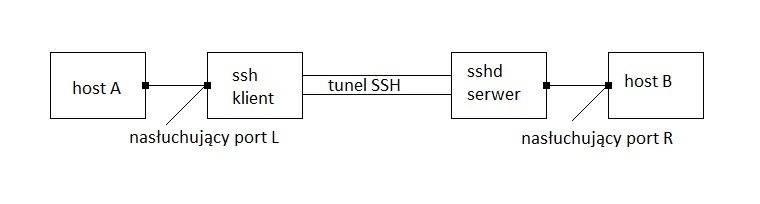
\includegraphics[width=12cm]{przekierowywanie_lokalne_SSH.jpg}
\caption{SSH lokalne przekierowywanie portu}\label{SSH}
\end{figure}

Host A wykonuje bezpiecznie połączenie do hostu B poprzez port R. Połączenie hostu A z hostem B przebiega w następujący sposób:
\begin{itemize}
\item host A łączy się do porty L na kliencie SSH,
\item SSH przekierowuje połączenie poprzez bezpieczny tunel do serwera SSH,
\item serwer SSH łączy się z hostem B poprzez port R.
\end{itemize}
\newpage
Port L na hoście A i port R na hoście B ustawione są w trybie ciągłego nasłuchiwania dla lokalnego połączenia. Na rys.~\ref{SSH_1} przedstawiono zdalne przekierowywanie portu z hosta B do hosta.
 
\begin{figure}[H]
\centering
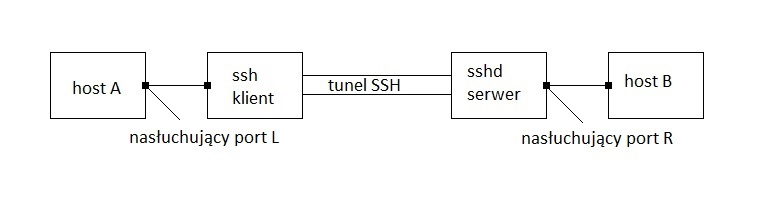
\includegraphics[width=12cm]{przekierowywanie_zdalne_SSH.jpg}
\caption{SSH zdalne przekierowywanie portu}\label{SSH_1}
\end{figure}

Zdalne przekierowanie portu przebiega w następujących krokach:
\begin{itemize}
\item klient SSH wysyła żądanie zdalnego przekazywania portów, co powoduje nasłuchiwanie połączeń na porcie R po stronie serwera,
\item przekierowanie połączenie przez bezpieczny tunel do klienta SSH,
\item klient SSH łączy się do hosta A poprzez nasłuchujący port L po jego stronie.
\end{itemize}
\quad 
Wykorzystując zjawisko tunelowania do prywatnej sieci wirtualnej tworzymy bezpieczne połączenie poprzez tunel między dwoma sieciami ~\cite{SSH}.

\subsubsection{IPsec}
\quad Protokół IPsec zawiera trzy główne pod protokoły:
\begin{itemize}
\item protokół uwierzytelnienie nagłówków (AH) - zapewnia uwierzytelnienie i integralność pakietów protokołu internetowego (IP),
\item  protokół bezpieczeństwa danych ESP - zapewnia te same usługi co protokół AH i dodatkowo zapewnia bezpieczeństwo danych,
\item protokół wymiany klucza internetowego IKE - zapewnia zarządzanie kluczem, umożliwiając bezpiecznie skojarzenie dwóch hostów.
\end{itemize}
\quad Protokoły AH i ESP mogą działać w dwóch trybach: transportowym i tunelowym. Tryb transportowy zapewnia bezpieczeństwo dla warstw powyżej datagramu IP. Jest on inicjowany głównie między dwoma stałymi hostami, połączenie nie może być nawiązana między dwoma sieciami lub między siecią i hostem. Zaś tryb tunelowy zapewnia bezpieczeństwo całego datagramu IP. Jest on stosowany do połączenia tunelowego między dwoma sieciami lub między hostem, a siecią. Na rys.~\ref{IPsec} poniżej przedstawiono schematyczny tryb tunelowy dla protokołu IPsec.

\begin{figure}[H]
\centering
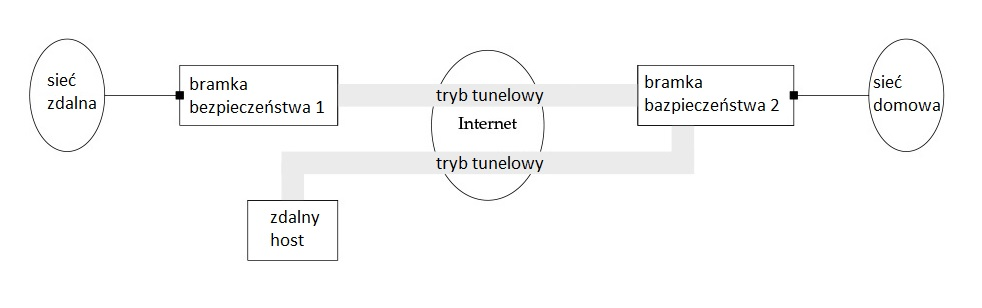
\includegraphics[width=15cm]{tryb_tunelowy_IPsec.jpg}
\caption{Tryb tunelowy IPsec}\label{IPsec}
\end{figure}
 
\quad Sieć zdalna jest połączona z siecią domową za pośrednictwem sieci tunelowej, bramki bezpieczeństwa 1 i bramki bezpieczeństwa 2. Funkcją bramek jest szyfrowanie, deszyfrowanie, zapobieganie ponownego odtwarzania wysyłanych pakietów i uwierzytelnianie. Z poziomu hostów bramki bezpieczeństwa i tunelowanie jest niewidoczne. Występują trzy metody uwierzytelnienia danych z udziałem protokołu bezpieczeństwa IPsec: wstępnie uzgodnione klucze, klucze prywatne i publiczne RSA oraz certyfikaty. Nagłówki uwierzytelniające dla trybu transportowego i tunelowego różnią się od siebie. Powszechny pakiet IP wchodzący w wyższą warstwę TCP składa się z: nagłówka IP, nagłówka TCP i danych użytkownika. Dla trybu transportowego nagłówek uwierzytelnienia dla IPsec składa się z: nagłówka IP, nagłówka uwierzytelniającego, nagłówka TCP i danych użytkownika. W tunelowym trybie nagłówek uwierzytelniający kopiuje część wewnętrzną nagłówka IP, która jest używana do utworzenia nowego zewnętrznego nagłówka IP. Nagłówek składa się z: zewnętrznego nagłówka IP, nagłówka uwierzytelniającego, wewnętrznego nagłówka IP, nagłówka TCP i danych użytkownika.

IPsec korzysta z protokołu Internet Key Exchange (IKE) w celu nawiązania i ustanowienie bezpiecznego połączenia między dwoma hostami lub zdalnego dostępu tunelowania VPN. Protokół IKE występuje w dwóch wersjach IKEv1 i IKEv2. Protokół IKEv1 można podzielić na dwie fazy, pierwsza w nich odpowiada za następujące funkcjonalności: algorytmy szyfrowania, algorytmy haszowania, algorytm Diffiego-Hellmana oraz metodę uwierzytelniania. Faza druga IKEv1 jest głównie używana do szyfrowania w protokole IPsec. Do szyfrowania wykorzystujemy algorytmy Data Encryption Standard (DES),  Triple DES o długości 168 bitów czy Advanced Encryption Standard (AES) o długości 128-256 bitów. Spośród wymienionych powyżej algorytmów DES zapewnia najniższe bezpieczeństwo danych, zaś AES o długości klucza 256 bitów największe bezpieczeństwo. Algorytmy haszujące zastosowane w protokole IPsec to: Secure Hash Algorithm (SHA) oraz Message Digest 5 (MD5). Protokół MD5 jest mniej bezpieczny niż algorytm SHA.
Kiedy używamy IPsec wraz z VPN przesyłane dane będą zabezpieczone podczas przesyłania, w celu uniemożliwienia atakującemu zdobycie jawnych danych. Proces szyfrowania, który zapewnia poufność przesyłanych danych nie daje możliwości łatwej modyfikacji wrażliwych danych atakującemu.

Do stworzenia protokołu zrzeszenia bezpieczeństwa(Security Association AS) dla IPsec używanych jest kilka komponentów, które służą do przetwarzania ruchu tekstu jawnego,który jest chroniony i następnie przekształcany w tekst zaszyfrowany. Te same komponenty są używane do odszyfrowania danych. Protokół IPsec korzysta z trzech baz danych: 
\begin{itemize}
\item baza danych zasad zabezpieczeń - Security Policy Database (SPD) określa jaki ruch ma być chroniony,
\item baza danych stowarzyszenia zabezpieczeń - Security Association Database (SAD) określa w jaki sposób ruch jest chroniony,
\item baza danych autoryzacji - Peer Authorization Database (PAD) zapewnia mechanizm wymuszający  politykę z oparciu o protokół IKE.
\end{itemize}

\subsubsection{Secure Socket Tunneling protocol Based on VPN}
\quad Protokół SSTP umożliwia administratorom na ustanowienie tunelów poprzez główną sieć korporacyjną na Windows Serwer. Dzięki zredukowanie wymaganych kroków technicznych do utworzenia tunelów między organizacjami zyskujemy niższy koszt administracyjny. Brak dodatkowych zmian w infrastrukturze dla protokołu SSTP, gdyż podobnie jak w protokóle HTTPS jest obsługiwana zapora sieciowa i serwery proxy. Protokół SSTP wykorzystuje protokołu SSL do transportu ruchu sieciowego. SSL jest certyfikatem odpowiedzialnym za poświadczenie wiarygodności domeny bądź jej właściciela, co zapewnia bezpieczeństw szyfrowania danych. PPP to protokół połączenia punkt-punkt. Protokołem odpowiedzialnym za sterowanie transmisją jest TCP. 
Proces utworzenia połączenia wykorzystującego VPN między klientem, a serwerem przebiega w następujący sposób:
\begin{itemize}
\item klient ustanawia połączenie TCP z serwerem SSTP pomiędzy dynamicznie zaalokowanym portem TCP po stronie klienta SSTP, a portem TCP 443 na serwerze SSTP,
\item klient SSTP wysyła wiadomość Witaj SSL świadczącą o chęci nawiązania połączenia SSL z serwerem SSTP,
\item serwer SSTP wysyła do klienta cyfrowy certyfikat,
\item klient SSTP sprawdza poprawność certyfikatu, wybiera metodę szyfrowania dla sesji SSL, generuje klucze i następnie szyfruje certyfikat serwera przy użyciu klucza publicznego,
\item klient SSTP wysyła zaszyfrowany klucz sesji SSL do serwera SSTP,
\item serwer SSTP odszyfrowuje zaszyfrowany klucz sesji SSL z wykorzystaniem klucza prywatnego; dalsza komunikacja klienta z serwerem jest zaszyfrowana wybraną metodą szyfrowania i odszyfrowywana kluczem sesji SSL,
\item klient wysyła komunikat HTTP poprzez sesję SSL do serwera,
\item klient ustala połączenie tunelowe z serwerem,
\item klient SSTP ustala połączenie PPP z serwerem SSTP, które obejmuje uwierzytelnienie danych logowanie użytkownika wraz z uwierzytelnieniem PPP i ustawieniem konfiguracji ruchu IP,
\item klient SSTP rozpoczyna proces ruchu sieciowego IP poprzez łącze PPP~\cite{SSTP}.
\end{itemize}

\subsubsection{L2TP}
\quad Protokół tunelujący warstwy 2 (Layer 2 Tunneling Protocol L2TP) działa na warstwie łączy danych, która jest drugą w siedmio warstwowym modelu odniesienia łączenia systemów otwartych (OSI). Protokół ten nie zapewnia szyfrowania ani poufności danych, z tego powodu jest często używany z protokołem IPsec, który zapewnia szyfrowanie i poufność danych. Protokół służy do komunikacji między klientem zwanym jako koncentrator dostępu L2TP(LAC) oraz serwerem nazywanym sieciowym serwerem L2TP (LNS). 
Protokół L2TP, który jest wykorzystywany do włączenie sieci VPN w Internecie jest rozszerzeniem protokołu PPTP. Powstał on w połączeniu protokołu firmy PPTP opracowanej przez Microsoft i L2F (przekierowywanie warstwy drugiej modelu OSI) firmy Cisco. Połączenie użytkownika domowego do sieci firmowej wykorzystujące protokół L2TP i połączenie internetowe przedstawiono w następujących krokach:
\begin{itemize}
\item zdalny użytkownik korzysta z analogowego połączenia telefonicznego lub łącza szerokopasmowego w celu zainicjowania połączenie PPP do dostawcy usług internetowych,
\item sieć LAC akceptuje połączenie co prowadzi do ustanowienia połączenia PPP,
\item w czasie gdy użytkownik końcowy i serwer nawiązują połączenie, koncentrator dostępu LAC rozpoczyna uwierzytelniania użytkownika metodą CHAP lub PAP,
\item po pomyślnie ukończonym procesie uwierzytelnienia, połączenie użytkownika z serwerem LNS zostaje pomyślnie nawiązane; w przypadku niepomyślnego procesu uwierzytelnienie klient uzyskuje dostęp do Internetu jako normalny użytkownik,
\item punkty końcowe tunelu (LAC i LNS) przed wysłaniem danych poprzez tunel uwierzytelniają się wzajemnie,
\item po utworzeniu tunelu VPN korzystającego z protokołu L2TP połączenie między użytkownikiem, a siecią korporacyjną zostaje nawiązane. 
\end{itemize}
Protokół L2TP jest protokołem sieci komputerowej wykorzystywanym przez dostawców internetowych do utworzenia wirtualnej sieci prywatnej między dwoma urządzeniami ~\cite{L2TP}.

\newpage
\section{Systemy wbudowane}
\subsection{Budowa }
\quad W obecnych czasach wbudowane systemy zyskają coraz większą popularność poprzez stosowanie ich w przedmiotach codziennego użytku między innymi: odkurzacz automatyczny, elektryczna hulajnoga, maszyny sprzedające, systemy alarmowe, telefony komórkowe czy drukarki. W przypadku niektórych zastosowań systemów wbudowanych np.telefony komórkowe czy systemy alarmowe niezbędne jest szyfrowanie występujących na nich wiadomości. W przypadku braku bloku kryptograficznego w systemie wbudowanym jest on podatny na atak. Przykładowo, w przypadku włamania do mieszkania z alarmem może on być wyłączony przez hakera w zdecydowanie krótszym czasie niż w przypadku takiego systemu alarmowego, na którym dane są całkowicie szyfrowane. Systemy wbudowane nie posiadają ściśle określonych architektur, projektowane są w zależności od zapotrzebowania bądź uniwersalne. Głównym argumentem przemawiającym za systemami wbudowanymi jest ich niski koszt produkcji oraz niski pobór mocy. Na rysunku~\ref{es} przedstawiono ogólny schemat blokowy komponentów zawartych wewnątrz mikrokontrolera.
\begin{figure}[H]
\centering
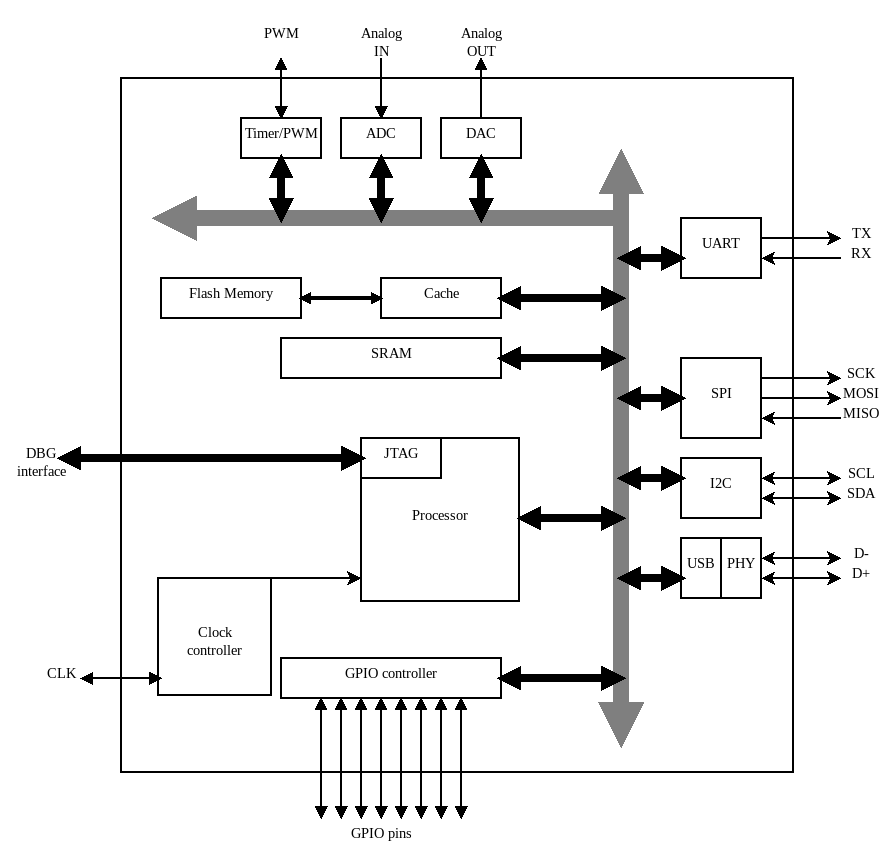
\includegraphics[width=11cm]{es.png}
\caption{Schemat blokowy komponentów wewnątrz ogólnego mikrokontrolera ~\cite{es}}.\label{es}
\end{figure}
W skład systemu wbudowanego wchodzą komponenty takie jak:

\paragraph{1. modulator szerokości impulsu PWM} \mbox{} \\

Modulator szerokości impulsów jest wykorzystywany do regulowania sygnału napięciowego lub prądowego przy stałej amplitudzie i częstotliwości. PWM jest wykorzystywany do kontrolowania mocy dostarczonej do urządzeń elektronicznych sterowanych przy pomocy mikrokontrolera. Wejściowy pulsujący sygnał jest generowany na sekwencyjne sygnały impulsowe w postaci fali o kształcie prostokątnym. Fala o charakterze prostokątnym posiada dwa stany: wysoki i niski, które są osiągalne poprzez przełączanie tranzystorów bądź tyrystorów w stan przewodzenia bądź zaporowy. Stan wysoki sygnały wyjściowego oznacza stan przewodzenia tranzystora, zaś stan niski oznacza stan zaporowy. Amplituda w sygnale prostokątnym jest to różnica między stanem wysoki, a stanem niskim napięcia w przypadku PWM sterowanego sygnałem napięciowym. Okres fali wyjściowej to czas trwania jego jednego cyklu, zaś częstotliwością fali jest odwrotność trwania okresu. Istotnym parametrem określającym wyjściową falę prostokątną jest również cykl roboczy, który jest stosunkiem procentowym czasu wysokiego stanu do okresu oznaczanego literą T.

\paragraph{2. przetwornik analogowo-cyfrowy A/C} \mbox{} \\

Przetwornik jest układem elektronicznym, który analogowy sygnał wejściowy konwertuje proporcjonalnie na cyfrowy sygnał wyjściowy. Proces ten polega na pomiarze wejściowego napięcia i jego zamiany na binarną wartość wyjściową. Jego zastosowanie można ujrzeć np. podczas mierzenia temperatury czy ważenia przedmiotów lub ludzi, gdzie sygnał analogowy jest zamieniany na cyfrowy i jego wartość jest interpretowana odpowiednio przez system wbudowany. 
Jednym z istotnych parametrów przetwornika jest jego rozdzielczość, która jest wyrażana w bitach. Przetwornik o rozdzielczości 8 bitów dla skali pomiarowej od 0 do 5 woltów ma rozdzielczość $2^{8}$ = 256, co można wyrazić w woltach jako $\frac{5-0}{256}$ = 19,53 mV. Innym przykładem rozdzielczości przetwornika jest 10 bitów, który dla skali 0 - 5 V ma rozdzielczość $2^{10}$ = 1024, co można wyrazić w woltach jako \mbox{$\frac{5-0}{1024}$ = 4,88 mV}. Jeśli zależy nam na lepszej jakości przetworzonego sygnały należy wybrać przetwornik o większej rozdzielczości. Jednym z etapów przetwornika jest próbkowanie, czyli przedstawienie sygnału ciągłego w postaci ciągu wartości, które są próbkami sygnału ciągłego. Po procesie próbkowania następuje proces kwantyzacji, który polega na przypisaniu wartości analogowej do najbliższego poziomu kwantyzacji. Dla przykładu w przypadku przetwornika o 3 bitowej rozdzielczości $2^{3} = 8$, występuje 8 poziomów kwantyzacji przedstawionych binarne na osi rzędnych jako wartości 000, 001, 010, 011, 100, 101, 110 i 111. W wielu przypadkach przetwornik z rozdzielczością 8, 10 czy 12 bitową jest wystarczający. W przypadku gdy sytuacja wymaga lepszego odwzorowania sygnału ciągłego należy wykorzystać przetwornik o większej rozdzielczości.
%rodzielczosc cos dodac o tym
%Przetwarzanie sygnału polega na jego próbkowaniu i kwantyzacji. Pró

%Nie wiem czy potocznie tak się to nazywa, ale nie jest to do końca precyzyjne stwierdzenie. Wejście to wejście, natomiast ADC to blok, który może być użyty, ale tylko gdy zależy nam na sygnale cyfrowym. W praktyce przed blokiem ADC powinno stosować się filtr antyaliasingowy, aby usunąć z sygnału analogowego składowe o  częstotliwościach większych niż połowa szybkości próbowania sygnału.    
\paragraph{3. przetwornik cyfrowo-analogowy C/A} \mbox{} \\

Przetwornik A/D jest układem elektronicznym, który konwertuje wejściowe dane binarne na analogowe dane wyjściowe. Jego zastosowanie można wykorzystać np. do sterowania silnika krokowego wyjściowym sygnałem napięciowym bądź wyświetlania godziny na zegarku analogowym.

\paragraph{4. wejścia/wyjścia ogólnego przeznaczenia GPIO (ang. general-purpose input/output)} \mbox{} \\


Wejścia-wyjścia ogólnego przeznaczenia są wykorzystywane do komunikacji użytkownika z systemem wbudowanym. W celu wykorzystania pinu wejścia/wyjścia ogólnego przeznaczenia należy odpowiednio go skonfigurować dla danego urządzenia.

\paragraph{5. uniwersalny odbiornik i nadajnik asynchroniczny UART} \mbox{} \\

Uniwersalny odbiornik i nadajnik asynchroniczny zwany jako UART(ang. universal asynchronous receiver-transmitter) służy do komunikowania się z systemem wbudowanym. Jest on jednym z powszechnie stosowanych protokołów komunikacyjnych. UART konwertuje równoległe dane na szeregowy strumień bitów danych. Komponent ten nie posiada zegara. Ramka wiadomości wykorzystywana do komunikacji z wykorzystaniem UART składa się z:
\begin{itemize}
\item bit początkowy sygnalizujący początek komunikacji,
\item bity danych,
\item bit parzystości, który jest wykorzystywany do wykrywania błędów występujących podczas komunikacji,
\item bit stopu, który informuje nas o końcu komunikacji.
\end{itemize} 

Na rysunku~\ref{es} symbolem TX(z ang. transmitted data) oznaczone są dane wyjściowe, natomiast symbolem RX(z ang. received data) oznaczono dane wejściowe. Komponent ten jest wykorzystywany np. do czytnika linii papilarnych, gdzie po zeskanowaniu odcisku dane są przesyłane poprzez komponent UART w celu dalszego ich przetworzenia.

\paragraph{6. magistrala} \mbox{} \\

Magistrale są wykorzystywane do przesyłania danych między urządzeniami występującymi w danym systemie wbudowanym. W zależności od sposobu przesyłania danych magistrale można podzielić na jednokierunkowe, gdzie przesył danych jest odbywa się tylko w jednym kierunku i dwukierunkowe, gdzie przesył danych odbywa się w dwóch kierunkach. Magistrale dwukierunkowe(ang.duplex) można podzielić na full duplex, gdzie przesyłanie danych odbywa się jednocześnie między urządzeniami oraz na half duplex, gdzie przesył danych między urządzeniami może odbywać się tylko w jednym kierunku w określonym czasie. Spośród magistrali wyróżniamy: 

\begin{description}
\item [6.1. ]szeregowy interfejs urządzeń peryferyjnych SPI

\quad SPI(ang. Serial Peripheral Interface) służy do komunikowania się urządzeń peryferyjnych tj. klawiatura, mysz, monitor, skaner, drukarka, mikrofon, głośnik czy kamera internetowa z centralną jednostką obliczeniową. Dzięki protokołowi pełnego dupleksu umożliwia on jednoczesne wysyłanie i odbieranie danych. SPI jest szybszy od protokołu I2C, lecz wynaga większej ilości połączeń w porównaniu z $I^{2}$C. Urządzenia komunikujące się między sobą określono jako master i slave. W SPI występuje jedno urządzenie, które ma charakter master i do kilkunastu urządzeń określanych jako slave. Urządzenie master jest w hierarchii wyżej od urządzenia slave, które jest jemu podporządkowane. Do przesyłania danych między urządzeniem  podlegającym(slavem), a głównym(master) wykorzystana jest linia MOSI(z ang. master out, slave in). Dane przesyłane między urządzeniem głównym, a podlegającym odbywają się na linii MISO(z ang. master in, slave out). Przesyłanie danych z urządzenia głównego do podlegającego i z urządzenia podlegającego do urządzenia głównego odbywa się w tym samym czasie, zgodnie z taktem zegara systemowego(SCK). Większość urządzeń SPI obsługuje przesył tylko 8 bitowych danych.

\item [6.2. ]$I^{2}$C

\quad Magistrala $I^{2}$C(ang. Inter-Integrated Circuit), komunikuje się między urządzeniami w sposób szeregowy i dwukierunkowy. $I^{2}$C oprócz pinów służących do uziemienia i zasilania korzysta tylko z dwóch dodatkowych pinów. Dwie dodatkowe linie oznaczono jako SDA i SCL. Linie do przesyłania danych oznaczono SDA, zaś linie zegara oznaczono SCL.

\item [6.3. ]USB, PHY

\quad USB jest magistralą komunikującą się w sposób szeregowy. Służy ona do przesyłania danych między urządzeniami bądź zasilania podłączonego urządzenia. Została ona zaprojektowania w celu standaryzacji magistrali przesyłających lub zasilających urządzenia peryferyjnych tj. klawiatura, urządzenia wskazujące czy monitor. USB posiada cztery piny: zasilający, dwa piny danych(D- i D+) oraz uziemiający. PHY jest to warstwa fizyczna modelu odniesienia łączenia systemów otwartych(OSI). PHY jest odpowiedzialne za połączenie warstwy łącza do kabla miedzianego lub światłowodu.

\end{description}
\newpage
\paragraph{7. zegar czasu rzeczywistego RTC} \mbox{} \\

Zegar czasu rzeczywistego służy do śledzenia aktualnego czasu i daty, które są wykorzystywane jako znacznik przypisujący danym plikom ich czas utworzenia czy ostatniej modyfikacji. Zegar jest zasilany własną niezależną baterią, co znaczy że działa on również gdy zasilanie nie jest doprowadzone go układu. Bateria zasilająca zegar posiada żywotność ponad 10 lat. Ważnym parametrem zegara jest jego częstotliwość. Częstotliwość zegara jest to ilość instrukcji wykonana w czasie jednej sekundy, więc im większa częstotliwość zegara, tym więcej instrukcji jest wykonanych w tej samej jednostce czasu.


\paragraph{8. centralna jednostka obliczeniowa(procesor)} \mbox{} \\

Głównym komponentem składowym centralnej jednostki obliczeniowej zwanej procesorem są tranzystory, które działają w oparciu o sygnały prądowe lub napięciowe. Tranzystory są ze sobą połączone w celu utworzenia bramek logicznych tj. AND, OR, NOT, NAND, NOR, EX-OR i EX-NOR. Bramka logiczna NOT posiada jedno wejście i jedno wyjście, gdy bitem wejściowym jest 0 to na wyjściu otrzymujemy 1, natomiast gdy bitem wyjściowym jest 1 na wyjściu otrzymano wartość 0. Natomiast pozostałe bramki logiczne posiadają dwa bity wejściowe oznaczone jako A i B oraz jeden bit wyjściowy oznaczony C. Ich zależności logiczne zostały przedstawione w poniższej tabeli~\ref{bramki_logiczne}.

\begin{table}[H]
\centering
\begin{tabular}{|c|c|c|c|c|c|c|c|} 
\hline
A& B& C[AND] & C[NAND] & C[OR] & C[NOR] & C[EX-OR] & c[EX-NOR]\\ \hline
0 & 0& 0& 1& 0& 1& 0& 1\\ \hline
0 & 1& 0& 1& 1& 0& 1& 0\\ \hline
1 & 0& 0& 1& 1& 0& 1& 0\\ \hline
1 & 1& 1& 0& 1& 0& 0& 1\\ \hline
\end{tabular}
\caption{Bramki logiczne.}\label{bramki_logiczne}
\end{table}

Procesor jest stworzony w biliona takich bramek logicznych, więc im więcej tranzystorów posiada procesor tym wyższa jest jego wydajność i moc obliczeniowa. Wydajność procesora jest również zależna częstotliwości jego zegara, więc im większa częstotliwość zegara tym wyższa wydajność procesora. Liczba operacji procesora jest proporcjonalna do częstotliwości zegara. Obecnie powszechne są procesory wielordzeniowe, czyli wiele procesorów będących na jednym chipie. Pozwala to na równoległe wykonywanie instrukcji procesora przez co zwiększona jest jego wydajność. W skład głównych komponentów procesora wychodzą jednostka arytmetyczno-obliczeniowa zwana ALU, jednostka sterująca, pamięć podręczna, pamięć główna, pamięć dyskowa oraz urządzenia wejścia i wyjścia. Procesory można podzielić za względu na architektura na 32 i 64 bitowe. Procesory jedno rdzeniowe z architekturą 32 bitową wykonują operację czytania lub pisania 32 bitów w jednej jednostce czasowej, natomiast procesory z architekturą 64 bity w jednej jednostce czasowej.  




\paragraph{9. interfejs debugowania JTAG} \mbox{} \\
%DBG interface

JTAG jest standardem IEEE 1149.1 do testowania połączeń oraz debugowania płytek drukowanych. Interfejs JTAG korzysta z pięciu linii sygnałowych: wejścia danych(TDI), wyjścia danych(TDO), wejścia sygnału zegarowego(TCK), wyboru trybu pracy(TMS) i zerowania(TRST). JTAG jest powszechnym interfejsem, który umożliwia komunikację zewnętrznego komputera z komponentami znajdującymi się na systemie wbudowanym.

\paragraph{10. pamięć} \mbox{} \\

Głównym zadaniem pamięci jest przechowywanie danych w postaci binarnej. Systemy wbudowane działają na dwóch stanach, gdzie stan wysoki odpowiada dodatniemu napięciowi, zaś stan niski jest reprezentowany przez napięcie zerowe. Stan wysoki oznaczamy jako 1 w notacji binarnej, zaś stan niski jako 0 w notacji binarnej. Rozmiar pamięci wyrażamy w bitach [b], bajtach [B], kilobajt [KB], megabajt [MB], gigabajt [GB] i terabajtach [TB]. Jednostka kilobajt jest równa 1024 bajt, 1 megabajt równa się 1024 kilobajtów, 1 gigabajt równy jest 1024 megabajtów, zaś 1 terabajt równy jest 1024 gigabajtów. Do pamięci zaliczamy:
\begin{description}

\item[10.1. ]statyczna pamięć o dostępie swobodnym SRAM(ang. Static Random Access Memory)

SRAM jest to pamięć statyczna o swobodnym dostępie. Jest to pamięć statyczna, gdyż dane zawarte na niej są tak długo jak długo jest zasilany układ. Pamięć SRAM jest pamięcią ulotną. Magistrale danych i adresów łączą bezpośrednio procesor z pamięcią SRAM. Pamięć SRAM jest szybsza od pamięci DRAM w operacjach odczytu i zapisu danych, co jest następstwem jej większej ceny. Pamięć SRAM często jest wykorzystywana jako pamięć podręczna lub pamięć wewnętrzna procesora ze względu na swoją szybkość. Jedną z wad pamięci SRAM jest to, że wymaga ona więcej mocy do działania przez co wytwarza więcej ciepła i wymaga lepszego chłodzenia w porównaniu w pamięcią DRAM. %Kontroler SRAM umożliwia wykonywanie kilku operacji między procesorem, a SRAM za jego pośrednictwem. Operacje wykonywane przez kontroler SRAM to: strobowanie adresu procesora, operacja odczytu i zapisu,    Jest to zezwolenie na wyjściu (OE) i zezwolenie na zapis (WE) do pamięci SRAM oraz potwierdzenie (ACK) do procesora, które musi pochodzić z wyjść strobowania adresu procesora (AS) i odczytu / zapisu (R / W). To jest zadanie kontrolera SRAM.

\item[10.2. ]pamięć podręczna procesora Cache

Procesor systemu wbudowanego nieustanie czyta i zapisuje informacje z jego pamięci podręcznej. Głównymi cechami pamięci podręcznej jest mały rozmiar, tymczasowość i ich szybkość. Pamięć podręczną dzielimy na dwa poziomy. Pamięć podręczna pierwszego poziomu oznaczona L1 znajduje się na procesorze i jest mniejsza od pamięci poziomu drugiego. Pamięć podręczna poziomu drugiego oznaczona L2 znajduję się między procesorem, a pamięcią główną i jest większa od pamięci L1. W niektórych przypadkach pamięć pierwszego L1 i drugiego poziomu L2 jest umieszczona razem w pamięci procesora oraz jest dodawany poziom trzeci L3 pamięci podręcznej. Poziomy pamięci podręcznej opisuje zależność L1$<$L2$<$L3. 

\item[10.3. ]pamięć flash

Pamięć flash jest pamięcią nieulotną, co znaczy, że po odłączeniu zasilania znajdujące się na niej dane nie zostaną utracone. Pamięci flash są powszechnie stosowane w kartach pamięci, pamięciach USB czy dyskach SSD.
\end{description}

%\paragraph{Rejestr} \mbox{} \\ % rejestr i rejsster specjalny
%\paragraph{Dekoder instrukcji} \mbox{} \\
%\paragraph{Rejestr SREG} \mbox{} \\
\paragraph{11. szyny danych, adresowe i sterowania} \mbox{} \\

Wszystkie wewnętrzne komponenty znajdujące się na systemie wbudowanym  do komunikacji używają trzech szyn. Szyna danych jest odpowiedzialna za przesyłanie danych między nimi, szyna adresowa odpowiedzialna jest za wysyłanie adresów, natomiast szyna sterowania jest odpowiedzialna za wysyłanie instrukcji między komponentami ~\cite{es}.


%\subsection{Architektura systemów wbudowanych}
%\quad Architekturę systemów wbudowanych możemy podzielić na architekturę zależną od struktury pamięci i zależną od typu instrukcji. Struktura pamięci : harwardzka, zmodyfikowana harwardzka i von-Neumanna. Typu instrukcji RISC i CISC.
%\subsubsection{Architektura harwardzka}
%\subsubsection{Zmodyfikowana architektura harwardzka}
%\subsubsection{Architektura von-Neumanna}
%\subsubsection{RISC - Recuded Instruction Set Computer}
%\subsubsection{CISC - Complex Instruction Set Computer}

\newpage
%\part{Część praktyczna}
\section{Projekt aplikacji konsolowej algorytmu DES na systemie wbudowanym}
%Później na samym początku pred punktem 4.1. bym napisał jeszcze że w części tej zawarto to czy tamto i że w kolejnych podrozdziałach kolejno omówiono np. częśc hardwarerową projektu itd.
\quad W części projektowej na wstępie w podrozdziale 4.1 omówiono część sprzętową wykorzystaną do implementacji algorytmu. W podrozdziale 4.2 opisano sposób połączenia NodeMCU v2 ESP8266 z środowiskiem programistycznym Arduino. Kolejnym krokiem było przedstawienie w podrozdziale 4.3 manualnych obliczeń, które wykorzystano następnie do potwierdzenia poprawnej implementacji algorytmu DES na ESP8266. Następnie w podrozdziale 4.4 części praktycznej porównano otrzymane wyniki pomiarów czasu szyfrowania i deszyfrowania wiadomości. W ostatniej części w podrozdziale 4.5 przedstawiono implementację algorytmy DES z wykorzystaniem łącza bezprzewodowego Wi-Fi oraz jej analizę.

\subsection{Charakterystyka ESP8266}

\quad Mikrokontroler składa się z płytki NodeMCU v2 oraz układ ESP8266. Układ ESP8266 z wbudowanym 32 bitowym układem RISC(zredukowany zestaw instrukcji) z takowanym zegarem 80MHz połączono 22 pinami do płytki. Głównymi komponentami moduł WiFi ESP8266 NodeMCU v2 są :
\begin{itemize}
\item moduł Wi-Fi ESP8266MOD, 2,4GHz, 802.11b/g/n,
\item stabilizator napięcia AMS1117 3.3 DN711,
\item konwerter USB-UART umożliwiający programowanie poprzez USB przy wykorzystaniu środowiska Arduino,
\item pamięć Flash 4MB,
\item 10 portów GIPO, które mogą obsługiwać magistrale PWN, I2C i l-wire,
\item wbudowane 10-bitowe ADC,
\item 10-bitowy przetwornik analogowo-cyfrowy,
\item antena PCB,
\item dwa przełączniki stanowe,
\item wejście mikro USB,
\item kondensator tantalu, dioda niebieska~\cite{esp8266}.
\end{itemize} 

\newpage
Do projektu wykorzystano płytkę NodeMCU v2 ESP8266, której przód przedstawiono na rysunku~\ref{esp}, zaś tył na rysunku~\ref{esp_1}. Numery na rysunku~\ref{esp} oznaczają:\\ 
1. moduł Wi-Fi ESP8266MOD 2,4GHz, 802.11b/g/n\\
2. stabilizator napięcia AMS1117 3.3 DN711\\
3. most USB-UART\\
4. przełącznik stanowy Flash\\
5. przełącznik stanowy RST\\
6. wejście mikro USB\\
7. kondensator tantalu 106C 516C1\\
8. dioda niebieska 0603\\

\begin{figure}[H]
\centering
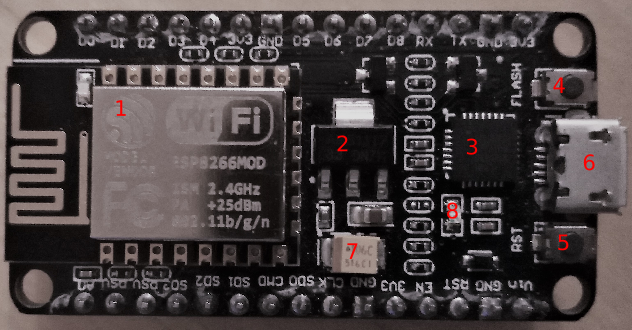
\includegraphics[width=10cm]{esp.png}
\caption{Przód mikrokontrolera NodeMCU v2 ESP8266.}\label{esp}
\end{figure}

\begin{figure}[H]
\centering
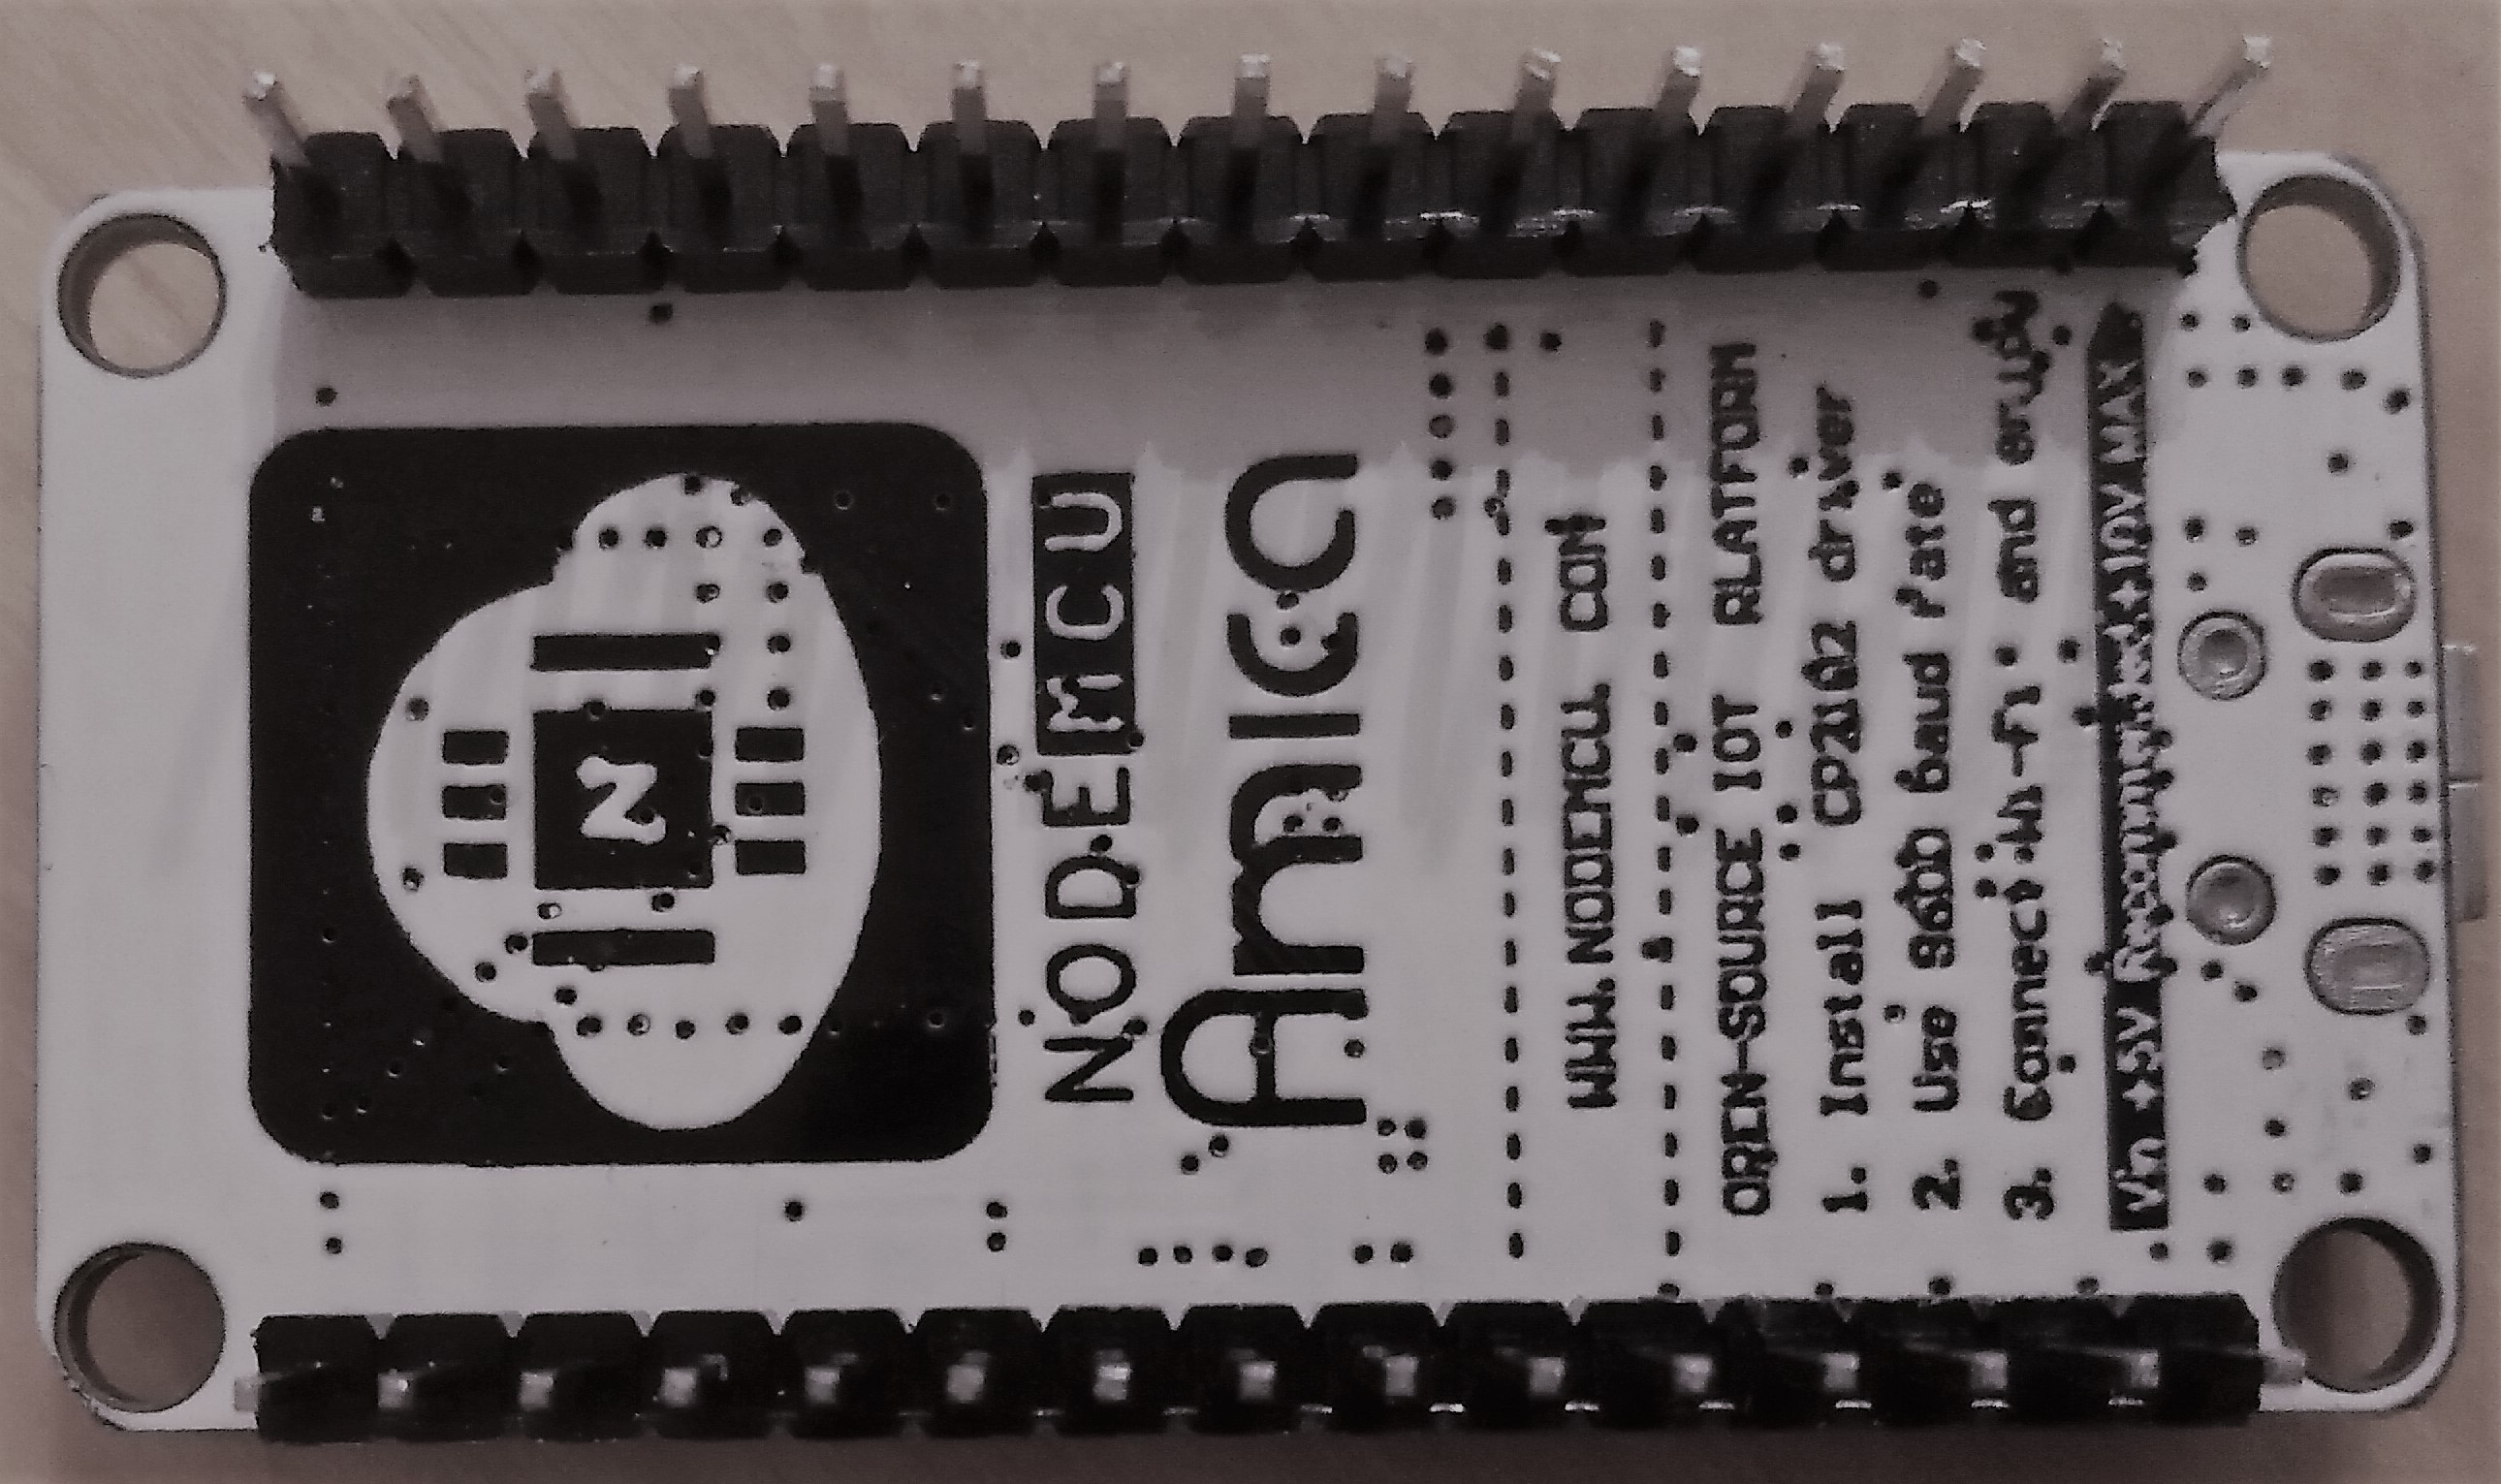
\includegraphics[width=10cm]{esp8266_1.jpg}
\caption{Przód mikrokontrolera NodeMCU v2 ESP8266.}\label{esp_1}
\end{figure}
\newpage
\subsection{Połączenie ESP8266 z Arduino}
Założenia projektowe:
\begin{itemize}
\item wykorzystanie mikrokontrolera ESP8266 NodeMCU v2,
\item wybrano język programowania C,
\item środowisko programistyczne Arduino uruchomione na systemie operacyjnym windows 10,
\item implementacja algorytmu DES na mikrokontrolerze,
\item pomiar czasu potrzebnego na szyfrowanie algorytmem DES,
\item pomiar czasu potrzebnego na deszyfrowanie algorytmem DES.
\end{itemize}


Podłączenie mikrokontrolera do środowiska programistycznego Arduino przebiegło w następujących krokach:
\begin{itemize}
\item pobranie i instalacja środowiska Arduino 1.8.7 IDE,
\item konfiguracja środowiska Arduino do obsługi ESP 8266 przez otwarcie okna dialogowego plik $\rightarrow$ preferencje i w miejscu "Dodatkowe adresy URL do menedżera płytek" umieszczenie adresu $http://arduino.esp8266.com/stable/package\char`_esp8266com\char`_index.json$ jak ukazano na rysunku~\ref{konf_arduino} znajdującym się poniżej,
\item instalacja paczki dla płytki ESP8266 poprzez otwarcie okna dialogowego narzędzia $\rightarrow$ Płytka $\rightarrow$ Menadżer płytek ... $\rightarrow$ wpisanie esp8266 w polu wyszukiwania i instalacja paczki,
\item konfiguracja płytki ESP826
\begin{itemize}
\item Narzędzia $\rightarrow$ Płytka $\rightarrow$ NodeMCU 1.0 (ESP-12E Module)
\item Narzędzia $\rightarrow$ Flash Size $\rightarrow$ 4M (3M SPIFFS)
\item Narzędzia $\rightarrow$ CPU Frequency $\rightarrow$ 80 Mhz
\item Narzędzia $\rightarrow$ Upload Speed $\rightarrow$ 921600
\item Narzędzia $\rightarrow$ Port $\rightarrow$ COM3.
\end{itemize} 
\end{itemize}

\begin{figure}[H]
\centering
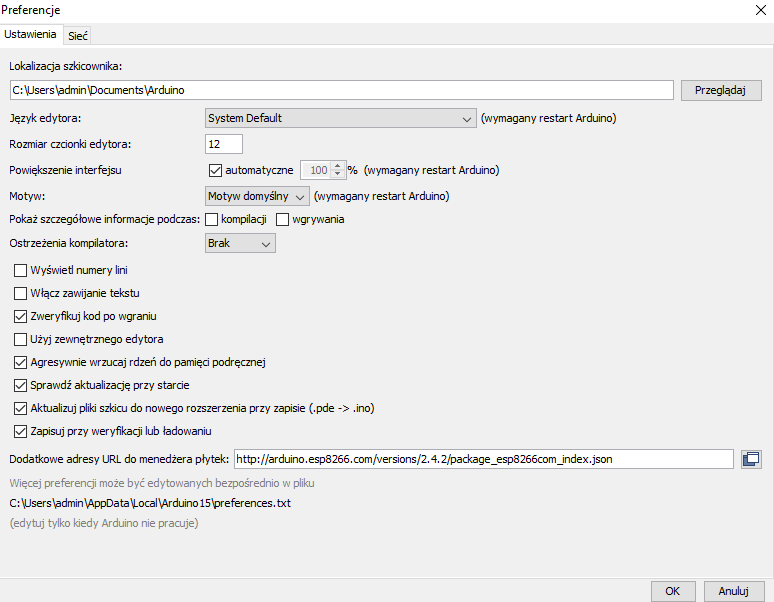
\includegraphics[width=12cm]{ustawienie_esp8266.png}
\caption{Konfiguracja środowiska Arduino dla płytki ESP8266.}\label{konf_arduino}
\end{figure}

W przypadku braku pewności, który port należy wybrać do komunikacji między środowiskiem Arduino, a płytką należy sprawdzić w menedżerze urządzeń. Na rysunku~\ref{mene} ukazano podgląd na menedżer urządzeń, w którego odczytujemy, że masz płytka podłączyła się z wykorzystaniem portu COM3.

\begin{figure}[H]
\centering
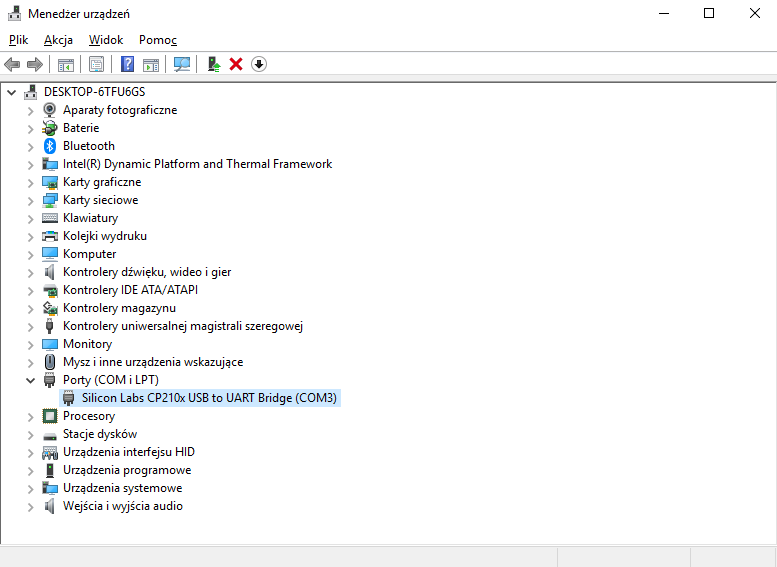
\includegraphics[width=12cm]{menedzer.png}
\caption{Konfiguracja środowiska Arduino dla płytki ESP8266.}\label{mene}
\end{figure}

Po zakończonej konfiguracji i zainstalowaniu paczki dla płytki ESP8266 niezbędna jest weryfikacja czy występuje poprawna komunikacja między płytką a środowiskiem Arduino. Na rysunku~\ref{wer_konf} przedstawiono pusty projekt w środowisku Arduino, który wykorzystano do weryfikacji komunikacji.

\begin{figure}[H]
\centering
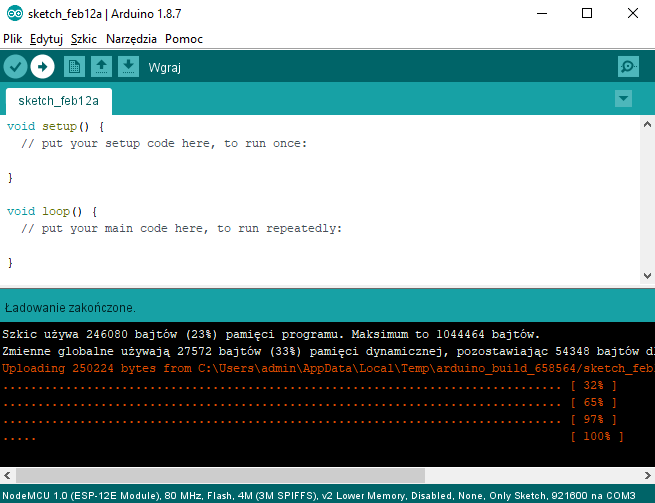
\includegraphics[width=12cm]{wer_instalacji.png}
\caption{Weryfikacja komunikacji środowiska Arduino z płytką ESP8266.}\label{wer_konf}
\end{figure}

W każdym programie niezbędne jest występowanie dwóch funkcji typu void, które nie zwracają żadnego argumentu. W funkcji setup umieszczamy kod, który ma być tylko uruchomiony jednorazowo. Funkcją główną programu jest void loop(), gdzie umieszczamy kod główny programu. Strzałka na białym tle służy do wgrania programu na płytkę. Weryfikacja komunikacji między płytką, a środowiskiem Arduino przebiegła pomyślnie o czym świadczy komunikat `Ładowanie zakończone`.

\subsection{Manualna implementacja algorytmu DES}

\quad W podrozdziale 2.4.1 zostały opisane teoretyczne kroki działania algorytmu DES, które zostały poniżej zobrazowane dla rundy pierwszej. W tabeli~\ref{binary} ukazano wiadomość w postaci decymalnej i heksadecymalnej oraz heksadecymalny klucz, które zostały użyte do przedstawienie działania algorytmu DES. 
 
\begin{table}[H]
\centering
\begin{tabular}{|c|c|c|c|c|c|c|c|c|}
\hline
wiadomość & witaj :)\\
\hline
wiadomość w postaci heksadecymalnej & 77 69 74 61 6A 20 3A 29\\
\hline
klucz & 43 23 66 A3 6B BB 53 C1\\
\hline
\end{tabular}
\caption{Dane wejściowe algorytmu DES.}~\label{binary}
\end{table}

Jednym z pierwszych kroków jest zamiana klucza heksadecymalnego do postaci binarnej co zostało ukazane w tabeli~\ref{klucz_to_binary}.


\begin{table}[H]
\centering
\begin{tabular}{|c|c|c|c|c|c|c|c|c|}
\hline
klucz & 4 & 3 & 2 & 3 & 6 & 6 & A & 3\\
\hline
klucz w postaci binarnej & 0100 & 001\textbf{1} & 0010 & 001\textbf{1} & 0110 & 011\textbf{0} & 1010 & 001\textbf{1}\\ 
\hline
numer bitu & 1-4 & 5-8 & 9-12 & 13-16 & 17-20 & 21-24 & 25-28 & 29-32\\
\hline
\hline
klucz & 6 & B & B & B & 5 & 3 & C & 1\\
\hline
klucz w postaci binarnej & 0110 & 101\textbf{1} & 1011 & 101\textbf{1} & 0101 & 001\textbf{1} & 1100 & 000\textbf{1}\\
\hline
numer bitu & 33-36 & 37-40 & 41-44 & 45-48 & 49-52 & 53-56 & 57-60 & 61-64\\
\hline
\end{tabular}
\caption{Klucz w postaci binarnej.}~\label{klucz_to_binary}
\end{table}

Po przekształceniu heksadecymalnego klucza do postaci binarnej usuwamy bit parzystości z 64 bitowego bloku czyli 8, 16, 24, 32, 40, 48, 56 i 64 bit. W tabeli~\ref{klucz_to_binary} bit parzystości oznaczono pogrubioną kursywą. Następnie z wykorzystaniem tabeli~\ref{per_klucza} dokonujemy przestawienie bitów klucza, odszukano bit 57 klucza, który wynosi 0 i wpisano do nowo utworzonej tabeli ~\ref{tabela_podstawienia} w lewym górnym rogu. W tak przedstawiony sposób dokonano translacji dla dalszych bitów klucza, a wynik przedstawiono w tabeli~\ref{tabela_podstawienia}.

\begin{table}[H]
\centering
\begin{tabular}{|c|c|c|c|c|c|c|c|c|c|c|c|c|c|c|c|c|}
\hline
permutacja klucza & 57 & 49 & 41 & 33 & 25 & 17 & 9 & 1 & 58 & 50 & 42 & 34 & 26 & 18 & &\\
\hline
numer bitu & 0 & 1 & 2 & 3 & 4 & 5 & 6 & 7 & 8 & 9 & 10 & 11 & 12 & 13 & 14 & 15\\
\hline
klucz binarny & 0 & 1 & 0 & 0 & 0 & 0 & 1 & 1 & 0 & 0 & 1 & 0 & 0 & 0 & 1 & 1\\
\hline
klucz po permutacji & 1 & 0 & 1 & 0 & 1 & 0 & 0 & 0 & 1 & 1 & 0 & 1 & 0 & 1 &&\\

\hline
\hline
permutacja klucza & 10 & 2 & 59 & 51 & 43 & 35 & 27 & 19 & 11 & 3 & 60 & 52 & 44 & 36 &&\\
\hline
numer bitu & 16 & 17 & 18 & 19 & 20 & 21 & 22 & 23 & 24 & 25 & 26 & 27 & 28 & 29 & 30 & 31\\
\hline
klucz binarny & 0 & 1 & 1 & 0 & 0 & 1 & 1 & 0 & 1 & 0 & 1 & 0 & 0 & 0 & 1 & 1\\
\hline 
klucz po permutacji & 0 & 1 & 0 & 0 & 1 & 1 & 1 & 1 & 1 & 0 & 0 & 1 & 1 & 0 &&\\

\hline
\hline
permutacja klucza & 63 & 55 & 47 & 39 & 31 & 23 & 15 & 7 & 62 & 54 & 46 & 38 & 30 & 22 &&\\
\hline
numer bitu & 32 & 33 & 34 & 35 & 36 & 37 & 38 & 39 & 40 & 41 & 42 & 43 & 44 & 45 & 46 & 47 \\
\hline
klucz binarny & 0 & 1 & 1 & 0 & 1 & 0 & 1 & 1 & 1 & 0 & 1 & 1 & 1 & 0 & 1 & 1 \\
\hline
klucz po permutacji & 0 & 1 & 1 & 1 & 1 & 1 & 1 & 1 & 0 & 0 & 0 & 0 & 0 & 1 &&\\

\hline
\hline
permutacja klucza & 14 & 6 & 61 & 53 & 45 & 37 & 29 & 21 & 13 & 5 & 28 & 20 & 12 & 4 &&\\
\hline
numer bitu & 48 & 49 & 50 & 51 & 52 & 53 & 54 & 55 & 56 & 57 & 58 & 59 & 60 & 61 & 62 & 63\\
\hline
klucz binarny & 0 & 1 & 0 & 1 & 0 & 0 & 1 & 1 & 1 & 1 & 0 & 0 & 0 & 0 & 0 & 1\\
\hline 
klucz po permutacji & 0 & 0 & 0 & 0 & 1 & 1 & 0 & 0 & 0 & 0 & 0 & 0 & 0 & 0 &&\\
\hline
\end{tabular}
\caption{Klucz w postaci binarnej.}~\label{tabela_podstawienia}
\end{table}


Klucz po permutacji z postaci 64 bitowej redukuje się do postaci 56 bitowej poprzez usunięcie bitów parzystości i dzieli na dwie części: prawą i lewą. W tabeli~\ref{LP} w górnym wierszy ukazane jest pierwsze 28 bitów klucza tzn. lewa część L oraz w dolnym wierszu przedstawiono następne 28 bitów klucza, które zwane są prawą częścią klucza P.

\begin{table}[H]
\centering
\begin{tabular}{|c|}
\hline
1010 1000 1101 0101 0011 1110 0110\\
\hline
0111 1111 0000 0100 0011 0000 0000\\
\hline
\end{tabular}
\caption{Obliczony klucz w postaci 56 bitowej.}\label{LP}
\end{table}

Klucz został podzielony na dwie osobne części, gdyż każda z nich podlega osobnym dalszym operacjom. W tabeli~\ref{shift} ukazano przesuniecie bitowe o 1 klucza w lewo wykonane na lewej i prawej części klucza.

\begin{table}[H]
\centering
\begin{tabular}{|c|c|c|c|c|c|c|c|}
\hline
klucz&0101 &0001 &1010& 1010& 0111& 1100 &1101\\
\hline
numer bitu&1-4 & 5-8 & 9-12&13-16&17-20&21-24&25-28\\
\hline
klucz&1111 &1110 &0000& 1000& 0110& 0000 &0000\\
\hline
numer bitu&29-32&33-36&37-40&41-44&45-48&49-52&53-56\\
\hline
\end{tabular}
\caption{Przesunięcie bitowe obliczonego klucza w postaci 56 bitowej.}\label{shift}
\end{table}

Ostatnim etapem obliczania klucza dla rundy pierwszej jest permutacja kompresji klucza DES zgodnie z tabelą~\ref{per_kompresji} kompresji klucza oraz przedstawienie wyniku w postaci heksadecymalnej co ukazano w tabeli~\ref{56}.

\begin{table}[H]
\centering
\begin{tabular}{ | p{3cm} | p{1.7cm} | p{1.7cm} | p{1.7cm} | p{1.7cm} | p{1.7cm} | p{1.7cm} |}
\hline
permutacja kompresji DES & 14 17 11 24  & 1 5 3 28 &  15 6 21 10 & 23  19 12 4 & 26 8 16 7 & 27 20 13 2\\ \hline
bitowy klucz 56bitowy po permutacji & 0010 & 0001 & 1010 & 0101 & 1100 & 0111 \\ \hline
heksadecymalny klucz 56bitowy po permutacji & 2 & 1 & A & 5 & C & 7\\
\hline \hline
permutacja kompresji DES & 41 52 31 37 & 47 55 30 40 & 51 45 33 48 & 44 49 39 56 & 34 53 46 42 & 50 36 29 32\\ \hline
bitowy klucz 56bitowy po permutacji & 1010 & 1010 & 0010 & 0000 & 1010 & 0011\\ \hline
heksadecymalny klucz 56bitowy po permutacji & A & A & 2 & 0 & A & 3\\ 
\hline
\end{tabular}
\caption{Permutacja klucza 56 bitowego.}\label{56}
\end{table}

Kluczem obliczonym dla pierwszej rundy jest 21A5C7AA20A3.\\


Następnym krokiem algorytmu jest przetworzenie w odpowiedni sposób jawnej wiadomości, którą przedstawiono w postaci heksadecymalnej i decymalnej w tabeli~\ref{wiadomosc}.

\begin{table}[H]
\centering
\begin{tabular}{|c|c|c|c|c|c|c|c|c|}
\hline
wiadomość heksadecymalna & 7 & 7 & 6 & 9 & 7 & 4 & 6 & 1\\ \hline
wiadomość binarna & 0111 & 0111 & 0110 & 1001 & 0111 & 0100 & 0110 & 0001\\ \hline
numer bitu & 1-4 & 5-8 & 9-12 & 13-16 & 17-20 & 21-24 & 25-28 & 29-32\\ \hline
wiadomość heksadecymalna & 6 & A & 2 & 0 & 3 & A & 2 & 9\\ \hline
wiadomość binarna & 0110 & 1010 & 0010 & 0000 & 0011 & 1010 & 0010 & 1001\\ \hline
numer bitu & 33-36 & 37-40 & 41-44 & 44-48 & 49-52 & 53-56 & 57-60 & 61-64\\ \hline
\end{tabular}
\caption{Wiadomość przedstawiona w postaci binarnej i heksadecymalnej.}\label{wiadomosc}
\end{table}

Następnym krokiem było dokonanie obliczenia permutacji początkowej wiadomości zgodnie z tabelą~\ref{per_poczatkowa} co ukazano w tabeli~\ref{per}.

\begin{table}[H]
\centering
\begin{tabular}{|c|c|c|c|c|c|c|c|c|c|}
\hline
wiadomość binarna po permutacji & 0001 & 1111 & 0100 & 0101 & 0000 & 0101 & 1000 & 1011\\ \hline
wiadomość heksadecymalna po permutacji & 1 & F & 4 & 5 & 0 & 5 & 8 & B\\ \hline
wiadomość binarna po permutacji & 0000 & 0000 & 1111 & 1111 & 1101 & 0010 & 0101 & 0001\\ \hline
wiadomość heksadecymalna po permutacji & 0 & 0 & F & F & D & 2 & 5 & 1\\ \hline

\end{tabular}
\caption{Transpozycja wiadomości w postaci binarnej z tabelą permutacji początkowej.}\label{per}
\end{table}



Lewa strona wiadomości to L = 1F45058B, prawa strona P = 00FFD251. 
Dla rundy pierwszej algorytmu lewą stroną wiadomości zostaje prawa część wiadomości, natomiast prawą część wiadomości obliczamy następująco:
\begin{itemize}
\item prawa część wiadomości podlega transpozycji zgodnie z tabelą~\ref{per_rozszerzenia} permutacji rozszerzenia,
\item operacja XOR wiadomości otrzymanej w wyniku transpozycji z obliczonym kluczem to EF108A230793,
\item prawa część wiadomości podlega transpozycji zgodnie z tabelą~\ref{per_rozszerzenia} permutacji rozszerzenia dając wynik przedstawiony w tabeli~\ref{per_rozszerzenia_wiadomosci}.
\end{itemize}

\begin{table}[H]
\centering
\begin{tabular}{|c|c|}
\hline
prawa część wiadomości & 00FFD251\\ \hline
& 0000 0000 1111 1111 1101 0010 0101 0001\\ \hline
permutacja rozszerzenia & 10000000 00010111 11111111 11101010 01000010 10100010\\ \hline
\end{tabular}
\caption{Permutacja rozszerzenia prawej części wiadomości.}\label{per_rozszerzenia_wiadomosci}
\end{table}

W tabeli~\ref{xor} przestawiono wynik operacji xor zmodyfikowanej wiadomości z kluczem.

\begin{table}[H]
\centering
\begin{tabular}{|c|c|}
\hline
wiadomość & 10000000 00010111 11111111 11101010 01000010 10100010\\ \hline
klucz & 00100001 10100101 11000111 10101010 00100000 10100011\\ \hline
XOR & 10100001 10110010 00111000 01000000 01100010 00000001\\ 
\hline
\end{tabular}
\caption{XOR wiadomości po permutacji rozszerzenia z kluczem.}\label{xor}
\end{table}

Następnym krokiem szyfrowania wiadomości było dokonanie podstawienia w S-blokach zgodnie z tabelą~\ref{s_bloki} s bloków. Wynik operacji XOR z tabeli ~\ref{xor} podzielono na S1 = 101000, S2 = 011011, S3 = 001000, S4 = 111000, S5 = 010000, S6 = 000110, S7 = 001000 i S8 = 000001. Wartości S bloków odczytano z użyciem tabeli~\ref{s_bloki}. Pierwszy w ostatni bit bloku oznacza rząd z tabeli~\ref{s_bloki} S-bloków, wartości 00 oznaczają wiersz 0, 01 oznaczają wiersz 1, 10 oznaczają wiersz 2, zaś 11 oznaczają wiersz 3. Dla wartości S1 pierwszy i ostatni bit bloku S1 = 10, co znaczy korzystanie z wiersza 2 i bloku S1. Następnie cztery bity między 1-5 bitem zmieniono na wartość decymalną. Dla S1 postać binarna 0100 wynosi 4 w postaci decymalnej, z tabeli~\ref{s_bloki} odczytujemy z wiersza 1, kolumny 4 wartość 14, więc S1 = 14. W sposób analogiczny odczytano pozostałe wartości S-bloków, które przedstawiono w tabeli~\ref{sbok_wynik}.
 
\begin{table}[H]
\centering
\begin{tabular}{|c|c|c|c|c|c|c|c|c|} 
\hline
decymalnie &14 &9& 6& 5& 8& 15& 15& 1\\ \hline
heksadecymalnie&D&9&6&5&8&F&F&1\\ \hline
binarnie & 1110& 1001& 0110& 0101& 1000& 1111& 1111& 0001\\ \hline
numer bitu &1-4 &5-8& 9-12& 13-16& 17-20& 21-24& 25-28& 29-32\\ \hline
\end{tabular}
\caption{Wiadomość po operacji na S blokach.}\label{sbok_wynik}
\end{table}

Jednym w ostatnich kroków szyfrowania wiadomości jest dokonanie transpozycji wyjścia S bloku z tabelą permutacji P-bloku~\ref{blok_P} w wyniku czego otrzymano: 1001 0011 1011 1001 1111 1100 0000 1111. Otrzymaną wartość poddano operacji XOR z lewą połową wiadomości (1F45058B), co przedstawiono jako (
0001 1111 0100 0101 0000 0101 1000 1011) $\oplus$ (
1001 0011 1011 1001 1111 1100 0000 1111) = 
1000 1100 1111 1100 1111 1001 1000 0100, co w postaci heksadecymalnej daje wartość 8CFCF984. Wartość prawej strony wiadomości dla rundy pierwszej wynosi 8CFCF984. Lewą częścią wynikową wiadomości jest niezmodyfikowana prawa część 32 bitowa wiadomości czyli 00FFD251.

\subsection{Implementacja algorytmu DES na ESP8266 z wykorzystaniem \mbox{połączenia} USB - mikroUSB}

\quad Algorytm DES zaimplementowano zgodnie z krokami przedstawionymi w manualnym obliczaniu szyfrowania algorytmem DES, którą szczegółowo przedstawionego na rysunku~\ref{des}. W celu poprawienia czytelności wyniku wypisywanego na monitor portu szeregowego poszczególne etapy pojedynczej rundy DES oznaczono jako krok 1, krok 2 itd. Na rysunku~\ref{runda_1} ukazano poszczególne kroki wyliczane z wykorzystaniem algorytmu DES. Tekst jawny oraz klucz wykorzystano taki sam jak w przykładzie manualnej implementacji DES. Poszczególne kroki oznaczają:
\begin{itemize}
\item Krok 1: Permutacja początkowa prawej części 32 bitowej wiadomości.
\item Krok 2: Permutacja początkowa lewej części 32 bitowej wiadomości.
\item Krok 3: Klucz po operacji permutacji klucza.
\item Krok 4: Przesunięcie bitowe klucza 56 bitowego.
\item Krok 5: Permutacja kompresji klucza 48 bitowego.
\item Krok 6: Permutacja rozszerzenia prawej części 32 bitowej wiadomości w wyniku, której otrzymano 48 bitową wiadomość.
\item Krok 7: Operacja XOR klucza danej rundy i prawej części 48 bitowej wiadomości.
\item Krok 8: Operacje na S blokach.
\item Krok 9: Operacja na P bloku.
\item Krok 10: Permutacja początkowa prawej części 32 bitowej wiadomości.
\item Krok 11: Permutacja początkowa lewej części 32 bitowej wiadomości.
\end{itemize}

\begin{figure}[H]
\centering
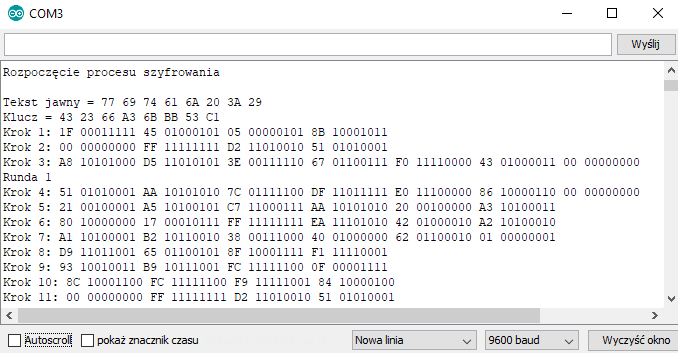
\includegraphics[width=12cm]{runda_1.jpg}
\caption{Wynik szyfrowania algorytmem DES dla rundy 1.}\label{runda_1}
\end{figure}
\newpage
Do zdefiniowania klucza oraz tekstu jawnego wykorzystano tablice, co ukazana na rysunku~\ref{klucz_tekst}.

\begin{figure}[H]
\centering
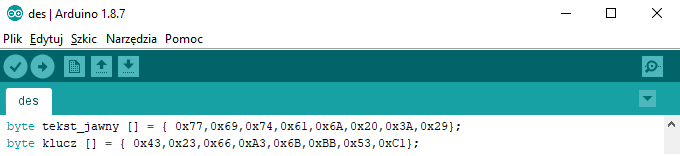
\includegraphics[width=12cm]{klucz_tekst.png}
\caption{Weryfikacja komunikacji środowiska Arduino z płytką ESP8266.}\label{klucz_tekst}
\end{figure}



Porównując wynik implementacji programu w środowisku Arduino na płytce NodeMCU v2 ESP8266 wraz z manualnym obliczeniem stwierdzono zgodność wyników dla rundy pierwszej algorytmu DES, co oznacza poprawną implementację algorytmu na mikrokontrolerze. Następnie dokonano pomiaru czasu szyfrowania i deszyfrowania wiadomości dla trzech prędkości szybkości transmisji danych, która jest określana w bitach na sekundę. Pomiarów dokonano dla szybkości transmisji: 9600, 19200 i 115200 bitów na sekundę. Szybkość transmisji danych mikrokontrolera określono poleceniem "Serial.begin(9600);", zaś w celu odczytania wyników na monitorze portu szeregowego ustawiono 9600. Pomiaru czasu szyfrowania i deszyfrowania wykonano z wykorzystaniem funkcji micros(), która zwraca czas wyrażony w mikrosekundach wykonywania programu. W celu obliczenia czasu szyfrowania i deszyfrowania obliczono różnicę czasu jako:\\
\begin{center}
unsigned long poczatek = micros();\\
szyfrowanie(tekst\_jawny, klucz);\\
unsigned long koniec = micros();\\
unsigned long czas\_szyfrowania = koniec - poczatek;\\
\end{center}

Pierwszym etapem było zmierzenie czasu szyfrowania i deszyfrowania dla przypadku, gdy dane obliczeń były wypisywane na monitor portu szeregowego. Na rysunku~\ref{9600_print},~\ref{19200_print} i ~\ref{115200_print} przedstawiono wyniki czasów w przypadku wypisywania poszczególnych kroków na konsole. Na rysunku~\ref{9600_print} przedstawiono wyniki czasu szyfrowania i deszyfrowania przy prędkości transmisji 9600 bitów na sekundę dla algorytmu wypisującego poszczególne kroki obliczeń na monitor portu szeregowego.

\begin{figure}[H]
\centering
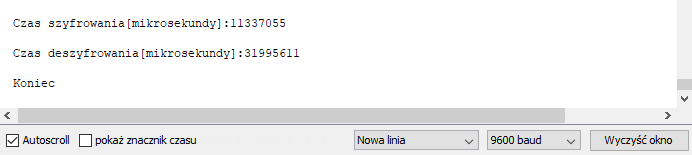
\includegraphics[width=12cm]{szy_desz_9600_print.png}
\caption{Czas szyfrowania i deszyfrowania dla prędkości transmisji danych 9600.}\label{9600_print}
\end{figure}

Na rysunku~\ref{19200_print} przedstawiono obliczony czas potrzebny do szyfrowania i deszyfrowania algorytmem DES dla prędkości transmisji danych 19200 bitów na sekundę dla algorytmu wypisującego poszczególne kroki obliczeń na monitor portu szeregowego. 

\begin{figure}[H]
\centering
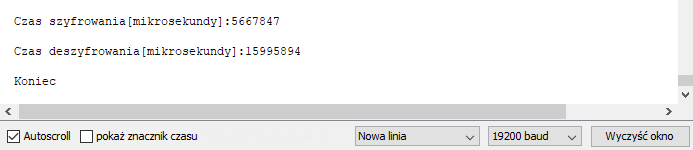
\includegraphics[width=12cm]{szy_desz_19200_print.png}
\caption{Czas szyfrowania i deszyfrowania dla prędkości transmisji danych 19200.}\label{19200_print}
\end{figure}

Na rysunku~\ref{115200_print} przedstawiono obliczony czas potrzebny do szyfrowania i deszyfrowania algorytmem DES dla prędkości transmisji danych 115200 bitów na sekundę dla algorytmu wypisującego poszczególne kroki obliczeń na monitor portu szeregowego.

\begin{figure}[H]
\centering
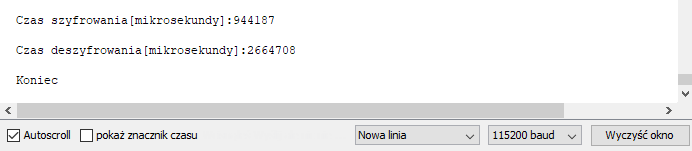
\includegraphics[width=12cm]{szy_desz_115200_print.png}
\caption{Czas szyfrowania i deszyfrowania dla prędkości transmisji danych 115200.}\label{115200_print}
\end{figure}

Drugim etapem było wyeliminowanie wypisywania na monitor portu szeregowego obliczeń poszczególnych kroków dla algorytmu DES i obliczenie rzeczywistego czasu zużytego na szyfrowania i deszyfrowanie wiadomości. Na rysunku~\ref{9600},~\ref{19200} i ~\ref{115200} przedstawiono wynik czasu obliczeń dla algorytmu DES dla różnych prędkości przesyłu transmisji danych. Na rysunku~\ref{9600} przedstawiono obliczone czas potrzebny do szyfrowania i deszyfrowania algorytmem DES dla prędkości transmisji danych 9600 bitów na sekundę.

\begin{figure}[H]
\centering
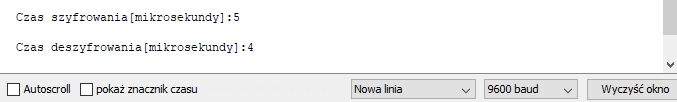
\includegraphics[width=12cm]{szy_desz_9600.png}
\caption{Czas szyfrowania i deszyfrowania dla prędkości transmisji danych 9600.}\label{9600}
\end{figure}

Na rysunku~\ref{19200} przedstawiono obliczone czas potrzebny do szyfrowania i deszyfrowania algorytmem DES dla prędkości transmisji danych 19200 bitów na sekundę.

\begin{figure}[H]
\centering
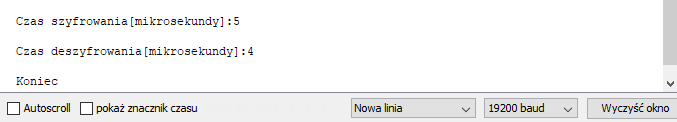
\includegraphics[width=12cm]{szy_desz_19200.png}
\caption{Czas szyfrowania i deszyfrowania dla prędkości transmisji danych 19200.}\label{19200}
\end{figure}

Na rysunku~\ref{115200} przedstawiono obliczone czas potrzebny do szyfrowania i deszyfrowania algorytmem DES dla prędkości transmisji danych 115200 bitów na sekundę.

\begin{figure}[H]
\centering
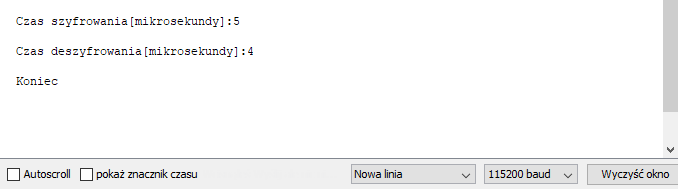
\includegraphics[width=12cm]{szy_desz_115200.png}
\caption{Czas szyfrowania i deszyfrowania dla prędkości transmisji danych 115200.}\label{115200}
\end{figure}

W tabeli~\ref{czas_przesylu} zobrazowano czas szyfrowania i deszyfrowania wiadomości 64 bitowej wyrażony w mikro sekundach. Szyfrowanie i deszyfrowanie wiadomości z wypisywaniem poszczególnych kroków na konsole konsumuje znacznie więcej czasu potrzebnego na poszczególne operacje. Możliwość podglądu poszczególnych kroków podczas procesu szyfrowania i deszyfrowania może być przydatna w celu wykrycia błędu występującego podczas wykonywania programu poprzez analizę otrzymanych wyników. Gdy zależy nam na wydajności oprogramowania szyfrującego należy unikać zbędnego wypisywania danych na konsolę, gdyż konsumuje to dużo czasu przez co wydajność oprogramowania maleje.  

\begin{table}[H]
\centering
\begin{tabular}{|c|c|c|c|}
\hline
prędkość transmisji [bit/s] &9600 &19200 &115200\\ \hline
szyfrowanie z wypisywaniem na konsole [$\mu$s]&11337055 &5667847 &944187\\ \hline
deszyfrowanie z wypisywaniem na konsole [$\mu$s]&31995611&15995894 &2664708\\ \hline
szyfrowanie [$\mu$s]&5&5&5\\ \hline
deszyfrowanie [$\mu$s]&4&4&4\\ \hline
\end{tabular}
\caption{Czas przesyłu danych przy wykorzystaniu algorytmu DES.}\label{czas_przesylu}
\end{table}

Na rysunku~\ref{czas_przesylu_procent} przedstawiono procentowy czas potrzebny do zaszyfrowania i odszyfrowania wiadomości 64 bitowej wykorzystując klucz 64 bitowy. 

\begin{figure}[H]
\centering
\begin{tikzpicture}
\begin{axis}[
    enlargelimits=0.15,
    legend style={at={(0.03,0.5)},anchor=west},
    ylabel={udział \% czasu [$\mu$s]},
    xlabel={prędkość transmisji[bit/s]},
    symbolic x coords={9600,19200,115200},
    xtick=data,
    ]
\addplot coordinates {(9600,100) (19200,100) (115200,100)};
\addplot coordinates {(9600,80) (19200,80) (115200,80)};
\legend{szyfrowanie,deszyfrowanie}
\end{axis}
\end{tikzpicture}
\caption{Procentowa prędkość przesyłu danych w zależności od prędkości transmisji.}\label{czas_przesylu_procent}
\end{figure}

Bit jest najmniejszą jednostką pamięci komputera oznaczoną literą b. Rozmiary pamięci komputera przedstawiono jako wielokrotności bitów i bajtów. Wielokrotność bita przedstawiono jako: 1Kb(kilobit) = 1024 bitów, 1Mb = 1048576 bitów, 1Gb = 1073741824 bitów itd. Wielokrotność bajta zaprezentowano jako 1KB(kilobajt) = 8192 bitów, 1MB = 8388608 bitów, 1GB = 8589934592 bitów itd. Dokonano pomiarów czasu szyfrowania i deszyfrowania danych o rozmiarach 1Kb, 8Kb i 16Kb dla trzech prędkości transmisji danych 9600, 19200 i 115200 bitów/s, które przedstawiono w tabeli~\ref{czas_przesylu_1K,8K}. 

\begin{table}[H]
\centering
\begin{tabular}{|c|c|c|c|}
\hline
prędkość transmisji [bit/s] &9600 &19200 &115200\\ \hline
szyfrowanie 1Kb[$\mu$s]&169&188&116\\ \hline
deszyfrowanie 1Kb[$\mu$s]&1718&113&101\\ \hline
szyfrowanie 8Kb[$\mu$s]&896&888&816\\ \hline
deszyfrowanie 8Kb[$\mu$s]&2417&813&801\\ \hline
szyfrowanie 16Kb[$\mu$s]&1697&1688&1616\\ \hline
deszyfrowanie 16Kb[$\mu$s]&3376&1613&1600\\ \hline
\end{tabular}
\caption{Czas przesyłu danych o rozmiarze 1Kb, 8Kb i 16Kb.}\label{czas_przesylu_1K,8K}
\end{table}

Na rysunku~\ref{czas_9600} przedstawiono czas szyfrowania i deszyfrowania wiadomości o rozmiarze 1Kb, 8Kb i 16Kb dla prędkości transmisji danych 9600bitów/s.

\begin{figure}[H]
\centering
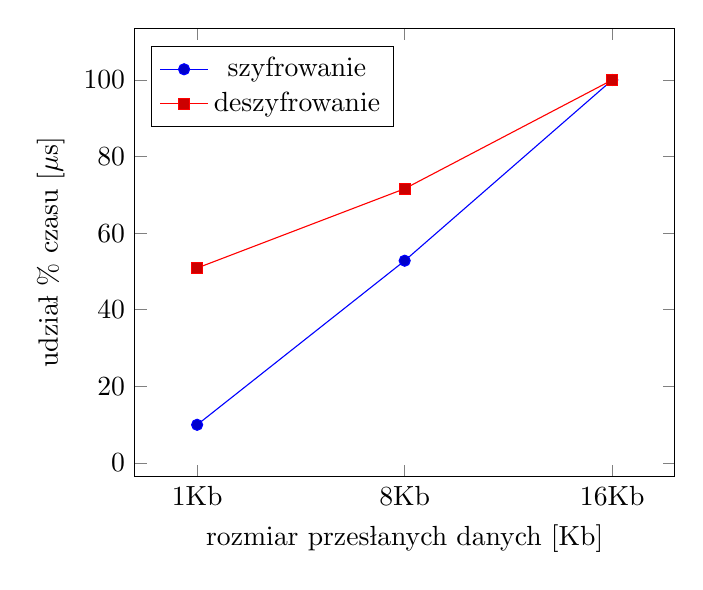
\begin{tikzpicture}
\begin{axis}[
    enlargelimits=0.15,
    legend style={at={(0.03,0.87)},anchor=west},
    ylabel={udział \% czasu [$\mu$s]},
    xlabel={rozmiar przesłanych danych [Kb]},
    symbolic x coords={1Kb,8Kb,16Kb},
    xtick=data,
    ]
\addplot coordinates {(1Kb,9.96) (8Kb,52.8) (16Kb,100)};
\addplot coordinates {(1Kb,50.89) (8Kb,71.6) (16Kb,100)};
\legend{szyfrowanie,deszyfrowanie}
\end{axis}
\end{tikzpicture}
\caption{Czas szyfrowania i deszyfrowania w zależności od rozmiaru danych dla prędkości transmisji 9600.}\label{czas_9600}
\end{figure}
\newpage
Na rysunku~\ref{czas_19200} przedstawiono czas szyfrowania i deszyfrowania wiadomości o rozmiarze 1Kb, 8Kb i 16Kb dla prędkości transmisji danych 19200bitów/s.

\begin{figure}[H]
\centering
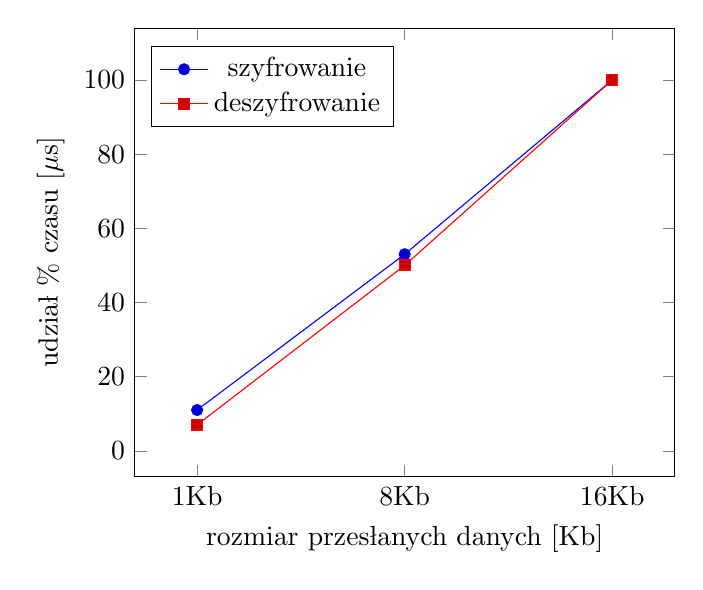
\begin{tikzpicture}
\begin{axis}[
    enlargelimits=0.15,
    legend style={at={(0.03,0.87)},anchor=west},
    ylabel={udział \% czasu [$\mu$s]},
    xlabel={rozmiar przesłanych danych [Kb]},
    symbolic x coords={1Kb,8Kb,16Kb},
    xtick=data,
    ]
\addplot coordinates {(1Kb,11) (8Kb,53) (16Kb,100)};
\addplot coordinates {(1Kb,7) (8Kb,50) (16Kb,100)};
\legend{szyfrowanie,deszyfrowanie}
\end{axis}
\end{tikzpicture}
\caption{Czas szyfrowania i deszyfrowania w zależności od rozmiaru danych dla prędkości transmisji 19200.}\label{czas_19200}
\end{figure}


Na rysunku~\ref{czas_115200} przedstawiono czas szyfrowania i deszyfrowania wiadomości o rozmiarze 1Kb, 8Kb i 16Kb dla prędkości transmisji danych 9600bitów/s.

\begin{figure}[H]
\centering
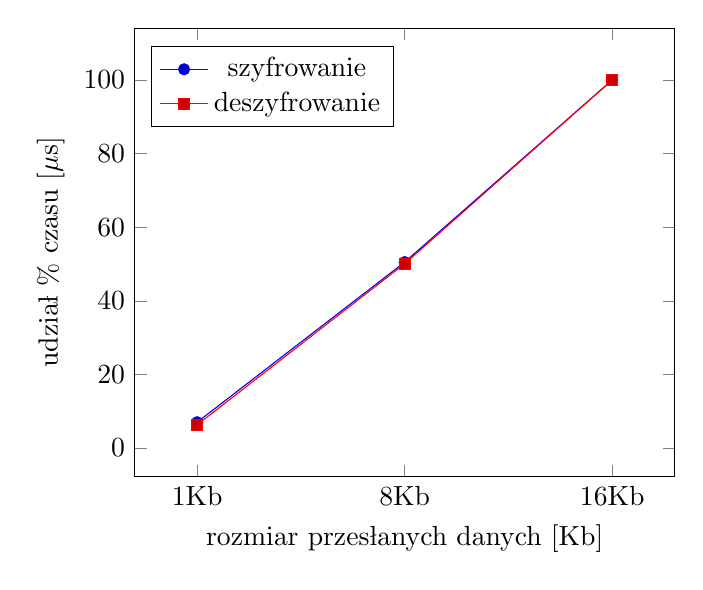
\begin{tikzpicture}
\begin{axis}[
    enlargelimits=0.15,
    legend style={at={(0.03,0.87)},anchor=west},
    ylabel={udział \% czasu [$\mu$s]},
    xlabel={rozmiar przesłanych danych [Kb]},
    symbolic x coords={1Kb,8Kb,16Kb},
    xtick=data,
    ]
\addplot coordinates {(1Kb,7) (8Kb,50.5) (16Kb,100)};
\addplot coordinates {(1Kb,6.3) (8Kb,50.06) (16Kb,100)};
\legend{szyfrowanie,deszyfrowanie}
\end{axis}
\end{tikzpicture}
\caption{Czas szyfrowania i deszyfrowania w zależności od rozmiaru danych dla prędkości transmisji 115200.}\label{czas_115200}
\end{figure}

Analizując rysunek~\ref{czas_9600},~\ref{czas_19200} i~\ref{czas_115200} spostrzeżono, że im większe prędkość transmisji danych tym bardziej czas szyfrowania jest zbliżony do czasu deszyfrowania danych. Dla najmniejszej prędkości przesyłu danych dostępnej w oprogramowaniu Arduino czas deszyfrowania wiadomości dla 1Kb i 8Kb jest większy niż czas potrzebny do zaszyfrowania tej wiadomości. Szyfrowanie DES wykorzystuje taki sam algorytm do deszyfrowania, w związku z czym czas szyfrowania i deszyfrowania  powinien być zbliżony. Jak widać na rysunku~\ref{czas_19200} i ~\ref{czas_115200} czas dla szyfrowania i deszyfrowania jest zbliżony, co świadczy o poprawnej implementacji algorytmu DES. Wydajność algorytmu można polepszyć poprzez wyeliminowanie z kodu zbędnych operacji. 

\subsection{Implementacja algorytmu DES na ESP8266 z wykorzystaniem modułu Wi-Fi}

\quad Płytka NodeMCU v2 posiada moduł Wi-Fi ESP8266MOD, który  wykorzystano do przesyłania danych. W celu wykonania połączenia Wi-Fi między ESP8266, a środowiskiem Arduino załączono bibliotekę ESP8266WiFi.h. Na rysunku~\ref{laczenie_wifi} pokazano niezbędne instrukcję do nawiązania połączenia bezprzewodowego. 

\begin{figure}[H]
\centering
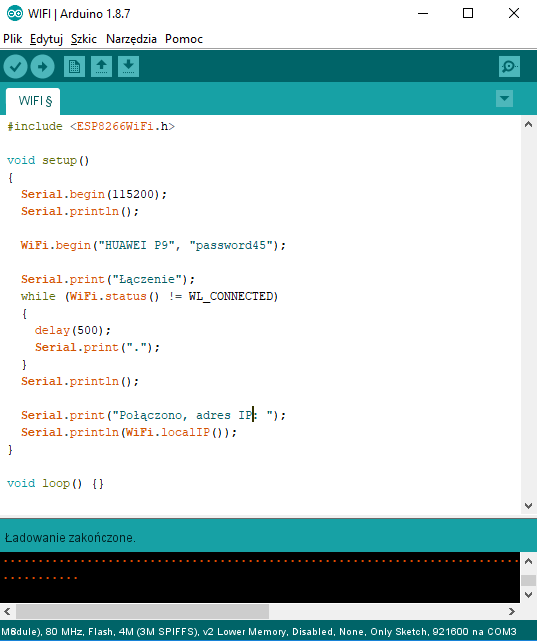
\includegraphics[width=9cm]{laczenie_wifi.png}
\caption{Nawiązanie połączenia bezprzewodowego z ESP8266.}\label{laczenie_wifi}
\end{figure}
\newpage
Instrukcja służąca do nawiązania połączenia z Internetem to WiFi.begin(nazwa sieci wifi, hasło). Na rysunku~\ref{polaczenie_wifi} przedstawiono wyjście z monitora portu szeregowego. Proces łączenia przebiegł pomyślnie.

\begin{figure}[H]
\centering
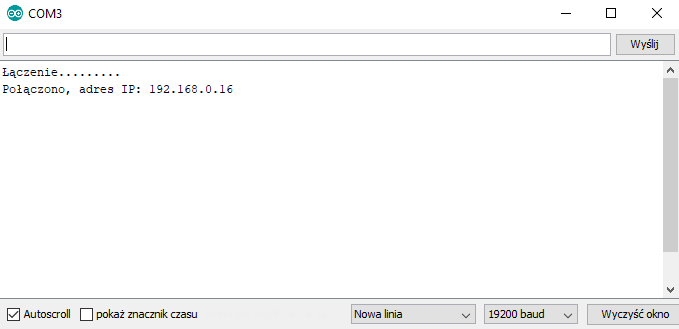
\includegraphics[width=12cm]{polaczenie_wifi.png}
\caption{Wynik nawiązanie połączenia bezprzewodowego z ESP8266.}\label{polaczenie_wifi}
\end{figure}

Dokonano pomiarów czasu szyfrowania i deszyfrowania w przypadku transmisji bezprzewodowej danych dla prędkości 9600, 19200 i 115200 z ich wypisywaniem na monitor portu szeregowego. Na rysunku~\ref{9600_wifi_print} przedstawiono czas szyfrowania i deszyfrowania dla bezprzewodowej transmisji o prędkości przesyłu 9600 bitów/s.

\begin{figure}[H]
\centering
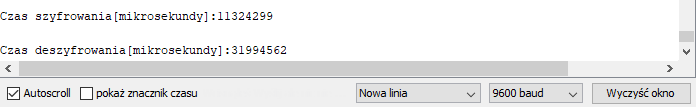
\includegraphics[width=12cm]{9600_wifi_print.png}
\caption{Czas szyfrowania i deszyfrowania dla bezprzewodowej transmisji danych 9600.}\label{9600_wifi_print}
\end{figure}

Na rysunku~\ref{19200_wifi_print} przedstawiono czas szyfrowania i deszyfrowania dla bezprzewodowej transmisji danych o prędkości przesyłu 19200 bitów/s.

\begin{figure}[H]
\centering
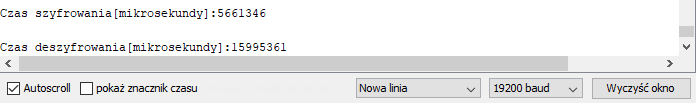
\includegraphics[width=12cm]{19200_wifi_print.png}
\caption{Czas szyfrowania i deszyfrowania dla bezprzewodowej transmisji danych 19200.}\label{19200_wifi_print}
\end{figure}

\newpage
Na rysunku~\ref{115200_wifi_print} przedstawiono czas szyfrowania i deszyfrowania dla bezprzewodowej transmisji danych o prędkości przesyłu 115200 bitów/s.

\begin{figure}[H]
\centering
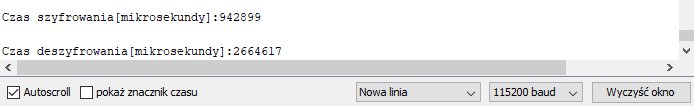
\includegraphics[width=12cm]{115200_wifi_print.png}
\caption{Czas szyfrowania i deszyfrowania dla bezprzewodowej transmisji danych 115200.}\label{115200_wifi_print}
\end{figure}


Dokonano pomiarów czasu szyfrowania i deszyfrowania w przypadku transmisji bezprzewodowej danych dla prędkości 9600, 19200 i 115200. Na rysunku~\ref{9600_wifi} przedstawiono czas szyfrowania i deszyfrowania dla bezprzewodowej transmisji o prędkości przesyłu 9600 bitów/s.

\begin{figure}[H]
\centering
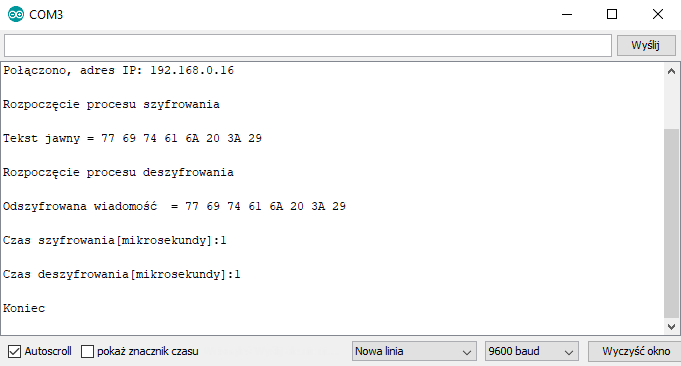
\includegraphics[width=12cm]{9600_wifi.png}
\caption{Czas szyfrowania i deszyfrowania dla prędkości bezprzewodowej transmisji danych 9600.}\label{9600_wifi}
\end{figure}

Na rysunku~\ref{19200_wifi} przedstawiono czas szyfrowania i deszyfrowania dla bezprzewodowej transmisji danych o prędkości przesyłu 19200 bitów/s.

\begin{figure}[H]
\centering
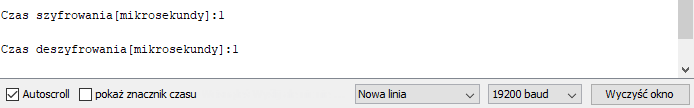
\includegraphics[width=12cm]{19200_wifi.png}
\caption{Czas szyfrowania i deszyfrowania dla prędkości bezprzewodowej transmisji danych 19200.}\label{19200_wifi}
\end{figure}

\newpage
Na rysunku~\ref{115200_wifi} przedstawiono czas szyfrowania i deszyfrowania dla bezprzewodowej transmisji danych o prędkości przesyłu 115200 bitów/s.

\begin{figure}[H]
\centering
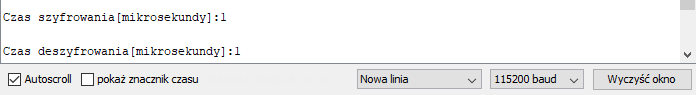
\includegraphics[width=12cm]{115200_wifi.png}
\caption{Czas szyfrowania i deszyfrowania dla prędkości bezprzewodowej transmisji danych 115200.}\label{115200_wifi}
\end{figure}

W tabeli~\ref{czas_przesylu_wifi} ukazano zmierzone czasy szyfrowania i deszyfrowania z wykorzystaniem transmisji bezprzewodowej Wi-Fi.



\begin{table}[H]
\centering
\begin{tabular}{|c|c|c|c|}
\hline
prędkość transmisji [bit/s] &9600 &19200 &115200\\ \hline
%usb
% 100% , 49,99, 8,33
%szyfrowanie z wypisywaniem na konsole [$\mu$s]&11337055 &5667847 &944187\\ \hline
% 100, 49,99, 8,33
%deszyfrowanie z wypisywaniem na konsole [$\mu$s]&31995611&15995894 &2664708\\ \hline

% 99,89, 49,93, 8,32
szyfrowanie z wypisywaniem na konsole [$\mu$s]&1132499 &5661346 &942899\\ \hline
% 99,99, 49,99, 8,33
deszyfrowanie z wypisywaniem na konsole [$\mu$s]&31994562&15995361 &2664617\\ \hline
%usb 5 -100%
%usb 4 - 80%
szyfrowanie [$\mu$s]&1&1&1\\ \hline% 1 -20%
deszyfrowanie [$\mu$s]&1&1&1\\ \hline
\end{tabular}
\caption{Czas przesyłu danych dla transmisji bezprzewodowej przy wykorzystaniu algorytmu DES.}\label{czas_przesylu_wifi}
\end{table}

Na rysunku~\ref{czas_przesylu_porownanie} ukazano zależność procentową czasu szyfrowania i deszyfrowania od prędkości transmisji z wykorzystaniem różnych łączy transmisji danych. Szyfrowanie i deszyfrowanie danych z wykorzystaniem transmisji przewodowej USB jest mniej wydajne niż w przypadku transmisji bezprzewodowej Wi-Fi.

\begin{figure}[H]
\centering
\begin{tikzpicture}
\begin{axis}[
    enlargelimits=0.15,
    legend style={at={(0.03,0.4)},anchor=west},
    ylabel={udział \% czasu [$\mu$s]},
    xlabel={prędkość transmisji[bit/s]},
    symbolic x coords={9600,19200,115200},
    xtick=data,
    ]
\addplot coordinates {(9600,100) (19200,100) (115200,100)};
\addplot coordinates {(9600,20) (19200,20) (115200,20)};
\addplot coordinates {(9600,80) (19200,80) (115200,80)};
\addplot coordinates {(9600,20) (19200,20) (115200,20)};

\legend{szyfrowanie USB,szyfrowanie Wi-Fi,deszyfrowanie USB, deszyfrowanie Wi-Fi}
\end{axis}
\end{tikzpicture}
\caption{Procentowa prędkość przesyłu danych w zależności od prędkości transmisji dla transmisji przewodowej i bezprzewodowej.}\label{czas_przesylu_porownanie}
\end{figure}

Na rysunku~\ref{szyf_wifi_usb} przedstawiono zależność czasu szyfrowania 64 bitowej wiadomości w przypadku wypisywania poszczególnych kroków algorytmu na monitor portu szeregowego od prędkości transmisji łącza przewodowego oraz bezprzewodowego.

\begin{figure}[H]
\centering
\begin{tikzpicture}
\begin{axis}[
    enlargelimits=0.15,
    legend style={at={(0.03,0.15)},anchor=west},
    ylabel={udział \% czasu [$\mu$s]},
    xlabel={prędkość transmisji[bit/s]},
    symbolic x coords={9600,19200,115200},
    xtick=data,
    ]
% 100% , 49,99, 8,33
% 99,89, 49,93, 8,32
\addplot coordinates {(9600,100) (19200,49.99) (115200,8.33)};
\addplot coordinates {(9600,99.89) (19200,49.93) (115200,8.32)};
\legend{szyfrowanie USB,szyfrowanie Wi-Fi}
\end{axis}
\end{tikzpicture}
\caption{Procentowa prędkość szyfrowania danych w zależności od prędkości transmisji dla transmisji przewodowej i bezprzewodowej.}\label{szyf_wifi_usb}
\end{figure}
\newpage
Na rysunku~\ref{deszyf_wifi_usb} przedstawiono zależność czasu deszyfrowania danych w przypadku wypisywania poszczególnych kroków algorytmu na monitor portu szeregowego od prędkości transmisji łącza przewodowego oraz bezprzewodowego. 


\begin{figure}[H]
\centering
\begin{tikzpicture}
\begin{axis}[
    enlargelimits=0.15,
    legend style={at={(0.03,0.15)},anchor=west},
    ylabel={udział \% czasu [$\mu$s]},
    xlabel={prędkość transmisji[bit/s]},
    symbolic x coords={9600,19200,115200},
    xtick=data,
    ]
% 100, 49,99, 8,33
\addplot coordinates {(9600,100) (19200,49.99) (115200,8.33)};
% 99,99, 49,99, 8,33
\addplot coordinates {(9600,99.99) (19200,49.99) (115200,8.33)};

\legend{deszyfrowanie USB, deszyfrowanie Wi-Fi}
\end{axis}
\end{tikzpicture}
\caption{Procentowa prędkość deszyfrowania danych w zależności od prędkości transmisji dla transmisji przewodowej i bezprzewodowej.}\label{deszyf_wifi_usb}
\end{figure}


Wyniki uzyskane na rysunku~\ref{szyf_wifi_usb} oraz ~\ref{deszyf_wifi_usb} ukazują, że czas szyfrowania i deszyfrowania 64 bitowej wiadomości dla łącza przewodowego i bezprzewodowego jest bardzo zbliżony do siebie. Natomiast wraz ze zwiększeniem prędkości transmisji czas szyfrowania i deszyfrowania skraca się, dzięki czemu osiągamy lepszą wydajność. Szyfrowanie z wykorzystaniem łącza bezprzewodowego Wi-Fi prezentuje lepszą wydajność w porównaniu do łącza przewodowego odbywającego się z wykorzystaniem kabla USB, co ukazuje rysunek~\ref{czas_przesylu_porownanie}. 

\newpage
\section{Wnioski}
\quad Celem pracy był opis algorytmów kryptograficznych, budowy systemów wbudowanych, implementacja algorytmu DES na module ESP8266 oraz pomiar czasu szyfrowania i deszyfrowania w zależności od rozmiary danych. W prezentowanej pracy magisterskiej jako element wprowadzający do kryptografii opisano działanie szyfrów strumieniowych, blokowych, symetrycznych i asymetrycznych. W części praktycznej niniejszej pracy dokonano implementacji algorytmu DES, który jest szyfrem symetrycznym, co oznacza, że istnieje jeden klucz do szyfrowania i odszyfrowywania przesyłanej wiadomości. Mikrokontrolerem wykorzystany do implementacji algorytmu była płytka ESP8266 NodeMCU v2, na którą wgrano oprogramowanie za pośrednictwem kabla mikro USB bądź wykorzystano łącze bezprzewodowe Wi-Fi i środowiska programistycznego Arduino. Pierwszym etapem było przedstawienie manualnej implementacji algorytmu DES dla pierwszej rundy w celu weryfikacji otrzymanych danych dla implementacji algorytmu na mikrokontrolerze. Stwierdzono poprawność implementacji algorytmu DES na ESP8266 po analizie wyników dla poszczególnych kroków rundy pierwszej wypisanych na monitorze portu szeregowego wraz z manualnymi obliczeniami. Otrzymane wyniki obliczeń manualnych są takie same jak obliczenia wykonane przy wykorzystaniu algorytmu na mikrokontrolerze ESP8266, co potwierdza poprawność implementacji.
 
\quad Drugim etapem części praktycznej pracy był pomiar i porównanie czasów szyfrowania i deszyfrowania wiadomości w zależności od rozmiaru przesyłanych danych oraz prędkości transmisji programu. Pomiarów czas szyfrowania i deszyfrowania wiadomości dokonano dla danych o rozmiarze 1 kilobit, 8 kilobitów i 16 kilobitów oraz dla trzech prędkości transmisji: 9600, 19200 i 115200 bitów/s. Otrzymane dane pozwalają stwierdzić, że dla większej prędkości transmisji danych czas szyfrowania i deszyfrowania danych jest niższy, co prowadzi do lepszej wydajności algorytmu. Dla wyższej prędkości transmisji czas szyfrowania i deszyfrowania jest zbliżony, co jest pożądanym zjawiskiem gdyż proces deszyfrowania przebiega przy wykorzystaniu takich samych operacji jak proces szyfrowania, lecz w odwrotnej kolejności. Proces szyfrowania i deszyfrowania również zwiększa się wprost proporcjonalnie do rozmiaru szyfrowanych danych. Obliczając ilość potrzebnego czasu do zaszyfrowania danych o rozmiarze 1Gb według 1000000000*116/1000=160000000[$\mu$s],otrzymujemy 1min. 56sek. W celu zaszyfrowania pliku o rozmiarze 1Gb potrzebujemy ok 2min., co jest czasem zadowalającym dla użytkowników domowych. Implementację algorytmu DES na ESP8266 oraz pomiar wydajności szyfrowania danych zrealizowano zgodnie z celem przedstawionym na początku pracy. 
%3. Później w podsumowaniu warto nawiązać do Celu i zakresu podkreślając co zostało zrobione, a co np. nie z podaniem powodów.


\newpage
\begin{thebibliography}{99}
%4
\bibitem{stream_cipher}  S. Bose, A. Kumar,
\emph{Cryptography and Network Security}
Pearson Education India, 03.2016, chapter 5
%10
\bibitem{DH} C. Chebbi
\emph{Advanced Infrastructure Penetration Testing},
Packt Publishing, 02.2018
%2
\bibitem{man_in_the_middle} E. Cole,
\emph{Hackers Beware},
08.2001, chapter Man-in-the-Middle Attack Against Key Exchange
%6
\bibitem{IDEA} T. Cui, H. Chen, L. Wen, M. Wang,
\emph{Cryptography and Communications: \mbox{Statistical} integral attack on CAST-256 and IDEA}, January 2018, Volume 10
%16
\bibitem{esp8266}Espressif Systems,
\emph{ESP8266-DevKitC Getting Started Guide}
Espressif Systems, 2018
%1
\bibitem{maskaraka} J. Forshaw,
\emph{
Attacking Network Protocols},
08.2017, chapter 4
%9
\bibitem{RSA} F.M. Groom, K. Groom and S.S. Jones
\emph{Network and Data Security for Non-Engineers},
\mbox{Auerbach} Publications, 08.2016, chapter 8
%8 
\bibitem{IDEAA} N. Hoffman,
\emph{Article in Cryptologia: A simplified IDEA algorithm},
Department of Mathematics, Northern Kentucky University, March 2007, str 143-151
%3
\bibitem{blok_cipher} Y. Li, Yu Sasaki, K. Sakiyama,
\emph{Security of Block Ciphers},
Wiley-IEEE Press, 04.2016, \mbox{chapter 1}
%15
\bibitem{es}D. Lacamera
\emph{Embedded Systems Architecture},
Packt Publishing, 05.2018
%12
\bibitem{SSH} A. Lockhart,
\emph{Network Security Hacks},
O'Reilly Media Inc., 04.2004, chapter 6

%14
\bibitem{L2TP} S. Malik,
\emph{Cover image for Network Security Principles and Practices
Network Security \mbox{Principles} and Practices},
Cisco Press, 10.2002
%7
\bibitem{asymetric}W. Mao,
\emph{Modern Cryptography: Theory and Practice}
Prentice Hall, 07.2003, chapter 8
%13
\bibitem{SSTP} J. Savill,
\emph{The Complete Guide to Windows Server 2008},
Addison-Wesley Professional, 10.2008, chapter 8
%11
\bibitem{PPTP} D. Stoddard i T.M. Thomas,
\emph{
Cover image for Network Security First-Step, Second Edition
Network Security First-Step, Second Edition},
Cisco Press, 12.2011, chapter 6
%5
\bibitem{DES} J. Wiley,
\emph{Information Security: Principles and Practice,2nd Edition},
M. Stamp, 05.2011, \mbox{chapter 3}





\end{thebibliography}
\newpage
\listoffigures
\addcontentsline{toc}{section}{Literatura}
\addcontentsline{toc}{section}{Spis rysunków}

\end{document}
